\chapter{Evaluation of the \textit{i}MGXS Scheme}
\label{chap:results}

The preceding chapter introduced a methodology for \textit{inferential multi-group cross section} (\textit{i}\ac{MGXS}) spatial homogenization. The \textit{i}\ac{MGXS} scheme uses unsupervised clustering algorithms to infer the optimal assignment of fuel pin instances to spatial homogenization tally zones based on an analysis of ``noisy'' \ac{MC} tally data. This chapter evaluates the \textit{i}\ac{MGXS} homogenization with respect to the scheme's two primary objectives:

\begin{itemize}[noitemsep]
\item Approach the \textbf{accuracy} of \textit{degenerate} spatial homogenization (Sec.~\ref{subsec:chap8-degenerate})
\item Approach the \ac{MC} \textbf{convergence} of \textit{null} spatial homogenization (Sec.~\ref{subsec:chap8-null})
\end{itemize}

\noindent Furthermore, the \textit{i}\ac{MGXS} scheme seeks to address the shortcomings of the Local Neighbor Symmetry (\ac{LNS}) spatial homogenization scheme (Sec.~\ref{sec:chap9-lns-homogenize}) -- namely, its inability to flexibly distinguish \ac{MGXS} clusters in arbitrary geometries (\textit{e.g.}, pins along assembly-assembly and assembly-reflector interfaces) and its poor scalability for large geometries.

The results presented in this chapter reflect the key observations made in Chaps.~\ref{chap:quantify} and~\ref{chap:spatial} for the null, degenerate and \ac{LNS} homogenization schemes. First, it was observed that pin-wise homogenization with track density-weighted \ac{MGXS} (Sec.~\ref{subsec:chap8-fiss-rates}) has no impact on the resultant eigenvalue since all schemes preserve global reactivity. In addition, it was shown that pin-wise \ac{MGXS} clustering must be accounted for to accurately predict pin-wise U-238 capture rates, but it is much less consequential for accurate fission rate predictions. These results inform the results and analysis presented in this chapter.

The accuracy of the \textit{i}\ac{MGXS} scheme is evaluated with respect to the null and degenerate schemes in Sec.~\ref{subsec:chap11-imgxs-results}. The analysis includes a presentation of the eigenvalue bias and the distributions of pin-wise U-238 capture rate errors for four clustering algorithms (Sec.~\ref{sec:chap10-train-predictor}) with varying numbers of clusters, for each of the six heterogeneous \ac{PWR} benchmarks (Sec.~\ref{sec:chap7-benchmarks}). The convergence rate of the OpenMOC solutions with the null, degenerate and \textit{i}\ac{MGXS} schemes is presented in Sec.~\ref{sec:chap11-converge} for ``noisy'' \ac{MC} tally data computed with varying numbers of particle histories. Sec.~\ref{sec:chap11-model-select} examines the empirical results for model selection criteria (Sec.~\ref{sec:chap10-model-select}) which may be use to select the most appropriate number of clusters for the \textit{i}\ac{MGXS} scheme. Finally, Sec.~\ref{sec:chap11-synthesis} concludes with an analysis of the computational resource requirements for a reference \ac{MC} calculation in comparison to deterministic multi-group calculations with the degenerate and \textit{i}\ac{MGXS} schemes necessary to reach a desired level of accuracy for pin-wise U-238 capture rates.


%%%%%%%%%%%%%%%%%%%%%%%%%%%%%%%%%%%%%%%%%%%%%%%%%%%%%%%%%%%%%%%%%%%%%%%%%%%%%%%%
\section{Multi-Group Results with \textit{i}MGXS}
\label{subsec:chap11-imgxs-results}

The \texttt{openmc.mgxs} module (Sec.~\ref{subsec:chap4-mgxs}) was used to compute 70-group \ac{MGXS} with OpenMC, along with all other tallies necessary to compute each of the features described in Sec.~\ref{sec:chap10-feature-extract}. In contrast to the \ac{MGXS} generated with OpenMC in Chaps.~\Crefrange{chap:quantify}{chap:unsupervised}, the \ac{MGXS} used in this chapter were generated with 10$\times$ more batches and 10$\times$ fewer histories per batch. The use of so many active batches made it possible to evaluate the convergence rate of the OpenMOC solutions in Sec.~\ref{sec:chap11-converge}\footnote{As a result of the different OpenMC runtime parameters used in this chapter, the OpenMOC eigenvalues and capture rate errors differ slightly from those reported in Chaps.~\Crefrange{chap:quantify}{chap:unsupervised}. The preceding chapters use 8 -- 9 $\times$ 10$^{8}$ active histories to generate \ac{MGXS}, while this chapter use 9.8 -- 9.9 $\times$ 10$^{8}$ active histories, since fewer histories are expended in the inactive cycles. Although so few istories per batch might risk under-sampling of the fission source distribution for a reference \ac{MC} calculation, it is less of a concern here since it is assumed that under-sampling is not as problematic for \ac{MGXS} generation.}. In particular, the OpenMC simulations were performed with 10,000 batches of 10$^{5}$ particle histories per batch for the assembly and colorset benchmarks, while 10$^{6}$ histories per batch were used for the quarter core \ac{BEAVRS} model. The fission source was converged with 200 inactive batches for the \ac{BEAVRS} model, while 100 inactive batches were employed for the other five benchmarks (Sec.~\ref{subsec:chap7-src-stationarity}). OpenMC's ``iso-in-lab'' feature (Sec.~\ref{subsec:chap4-iso-in-lab}) was employed to enable consistent comparisons between OpenMC's reference results and OpenMOC's calculations with an isotropic in lab scattering source.

%-how many batches for full core??

The 70-group \ac{MC} tally data was condensed to 2-groups for feature extraction within the \textit{i}\ac{MGXS} data processing pipeline. The litmus-only feature selection approach used the nuclide fraction thresholding litmus test (Sec.~\ref{subsubsec:chap10-litmus-nuc-frac}) to select the ``best'' reaction type for each pair of nuclides and energy groups, for each nuclide in the fuel and both energy groups. All available features were used for each selected reaction type, nuclide and energy group. No dimensionality reduction techniques (Sec.~\ref{sec:chap10-dimension-reduce}) were applied to the selected features. The $k$-means, agglomerative, BIRCH and Gaussian Mixture Model (GMM) clustering algorithms were separately used to train predictors for varying numbers of clusters (Sec.~\ref{sec:chap10-train-predictor}) to inform pin-wise spatial homogenization.

Each of the six benchmarks was modeled with OpenMOC using \ac{MGXS} generated by the \textit{i}\ac{MGXS} spatial homogenization scheme with the same runtime parameters as those used in Chap.~\ref{chap:quantify} for infinite, null and degenerate homogenization, and in Chap.~\ref{chap:spatial} for \ac{LNS} homogenization. The eigenvalue bias is presented in Sec.~\ref{subsec:chap11-imgxs-eigenvalues}, while the U-238 capture rate errors are analyzed in Sec.~\ref{subsec:chap11-imgxs-capt-rates}. Since \ac{MGXS} clustering was quantified to be largely inconsequential for fission rate predictions, the pin-wise fission rate errors for the \textit{i}\ac{MGXS} scheme are not considered here for brevity.

%%%%%%%%%%%%%%%%%%%%%%%%
\subsection{Eigenvalues}
\label{subsec:chap11-imgxs-eigenvalues}

The OpenMOC eigenvalues were compared to the reference OpenMC eigenvalues from Tab.~\ref{table:chap7-ref-eigenvalues}. The eigenvalue bias $\Delta\rho$ was computed from Eqn.~\ref{eqn:chap5-delta-rho} in units of \ac{pcm}. The bias is listed in Tab.~\ref{table:chap11-eigenvalues} for each benchmark, and varying numbers of clusters for each clustering algorithm. The same trends highlighted in Sec.~\ref{subsec:chap8-eigenvalues} observed from the null and degenerate biases in Tab.~\ref{table:chap8-openmoc-eigenvalues} remain true for \textit{i}\ac{MGXS} spatial homogenization. The \textit{i}\ac{MGXS} eigenvalues are within 10 \ac{pcm} of those computed with both null and degenerate homogenization for all benchmarks. As previously noted in Sec.~\ref{subsec:chap8-eigenvalues}, this is expected since the \ac{MGXS} for the null, degenerate and \textit{i}\ac{MGXS} schemes are homogenized from the same flux and should preserve globally-integrated reaction rates. Hence, neither the type of clustering algorithm nor the number of clusters is expected to systematically impact OpenMOC's eigenvalue predictions. Nevertheless, the consistent eigenvalue biases do support the conclusion that the \textit{i}\ac{MGXS} scheme is properly implemented.

\begin{table}[ht!]
  \centering
  \caption[OpenMOC eigenvalue bias for litmus-only feature selection]{OpenMOC eigenvalue bias $\Delta\rho$ for \textit{i}\ac{MGXS} spatial homogenization.}
  \small
  \label{table:chap11-eigenvalues}
  \vspace{6pt}
  \begin{tabular}{l l R{1.2cm} R{1.2cm} R{1.2cm} R{1.2cm} R{1.2cm} R{1.2cm}}
  \toprule
  \rowcolor{lightgray}
  & \multicolumn{1}{c}{\cellcolor{lightgray} \bf Clustering} & \multicolumn{6}{S[table-format=6.1]}{\cellcolor{lightgray} \textbf{\# Clusters}} \\
  \multirow{-2}{*}{\cellcolor{lightgray} \bf Benchmark} &
  \multicolumn{1}{c}{\cellcolor{lightgray} \bf Algorithm} &
  \multicolumn{1}{c}{\cellcolor{lightgray} \bf 1\footnotemark} &
  \multicolumn{1}{c}{\cellcolor{lightgray} \bf 2} &
  \multicolumn{1}{c}{\cellcolor{lightgray} \bf 4} &
  \multicolumn{1}{c}{\cellcolor{lightgray} \bf 8} &
  \multicolumn{1}{c}{\cellcolor{lightgray} \bf 16} &
  \multicolumn{1}{c}{\cellcolor{lightgray} \bf \# pins\footnotemark} \\
  \midrule
\multirow{4}{*}{\parbox{2.5cm}{1.6\% Assm}} & Agglomerative & \multirow{4}{*}{-168} & -168 & -168 & -168 & -168 & \multirow{4}{*}{-168} \\
& BIRCH & & -168 & -168 & -168 & -168 & \\
& \ac{GMM} & & -168 & -168 & -168 & -168 & \\
& $k$-means & & -168 & -168 & -168 & -168 & \\
  \midrule
\multirow{4}{*}{\parbox{2.5cm}{3.1\% Assm}} & Agglomerative & \multirow{4}{*}{-194} & -194 & -194 & -194 & -194 & \multirow{4}{*}{-194} \\
& BIRCH & & -194 & -194 & -194 & -194 & \\
& \ac{GMM} & & -194 & -194 & -194 & -194 & \\
& $k$-means & & -194 & -194 & -194 & -194 & \\
  \midrule
\multirow{4}{*}{\parbox{2.5cm}{3.1\% Assm w/ 20 \acp{BP}}} & Agglomerative & \multirow{4}{*}{-240} & -237 & -236 & -235 & -235 & \multirow{4}{*}{-235} \\
& BIRCH & & -237 & -236 & -235 & -235 & \\
& \ac{GMM} & & -236 & -235 & -236 & -235 & \\
& $k$-means & & -236 & -236 & -236 & -235 & \\
  \midrule
\multirow{4}{*}{\parbox{2.5cm}{2$\times$2 Colorset}} & Agglomerative & \multirow{4}{*}{-191} & -189 & -189 & -189 & -189 & \multirow{4}{*}{-188} \\
& BIRCH & & -189 & -189 & -189 & -188 & \\
& \ac{GMM} & & -188 & -189 & -188 & -189 &  \\
& $k$-means & & -188 & -189 & -188 & -189 & \\
  \midrule
\multirow{4}{*}{\parbox{2.5cm}{2$\times$2 Colorset w/ Reflector}} & Agglomerative & \multirow{4}{*}{-141} & -136 & -136 & -134 & -129 & \multirow{4}{*}{-141} \\
& BIRCH & & -138 & -137 & -136 & -132 & \\
& \ac{GMM} & & -136 & -136 & -137 & -132 & \\
& $k$-means & & -136 & -136 & -134 & -132 & \\
  \midrule
\multirow{4}{*}{\parbox{2.5cm}{BEAVRS Full Core}} & Agglomerative & \multirow{4}{*}{-122} & & -120 & -119 & -119 & \multirow{4}{*}{-116} \\
& BIRCH & &  & -120 & -120 & -119 & \\
& \ac{GMM} & & & -119 & -118 & -119 & \\
& $k$-means & & & -120 & -119 & -119 & \\
  \bottomrule
\end{tabular}
\end{table}

\addtocounter{footnote}{-2}
\stepcounter{footnote}
\footnotetext{\label{null}Null homogenization is equivalent to \textit{i}\ac{MGXS} homogenization with a single cluster.}

\stepcounter{footnote}
\footnotetext{\label{degenerate}Degenerate homogenization is equivalent to \textit{i}\ac{MGXS} homogenization with a cluster for each fuel pin.}

\vspace{-0.05in}

\begin{emphbox}
\textbf{The OpenMOC eigenvalues for \textit{i}\ac{MGXS} homogenization are consistent to within 10 \ac{pcm}  for all numbers of clusters due to the preservation of global reactivity.}
\end{emphbox}

\clearpage

%%%%%%%%%%%%%%%%%%%%%%%%%%%%%%%%
\subsection{U-238 Capture Rates}
\label{subsec:chap11-imgxs-capt-rates}

The OpenMOC energy-integrated pin-wise U-238 capture rates were compared to the reference OpenMC capture rates for \textit{i}\ac{MGXS} homogenization to compute the percent relative errors for each pin's capture rates. Sec.~\ref{subsec:chap11-imgxs-capt-rates-num-clusters} investigates the dependence of the maximum and mean errors with the number of clusters, while Sec.~\ref{subsec:chap11-imgxs-capt-rates-benchmark} compares the errors between null, degenerate and \textit{i}\ac{MGXS} homogenization. Sec.~\ref{subsec:chap11-imgxs-capt-rates-space-distrib} illustrates the spatial distributions of U-238 capture rate errors. Finally, Sec.~\ref{subsec:chap11-imgxs-capt-rates-compare} compares OpenMOC's U-238 capture rate predictions for different clustering models to understand relative impact of clustered \ac{MGXS} for different types of fuel pins.

%%%%%%%%%%%%%%%%%%%%%%%%%%%%%%%%%%%%%%%%%%%%%%%%%%%%%
\subsubsection{Variation with the Number of Clusters}
\label{subsec:chap11-imgxs-capt-rates-num-clusters}

This section compares the U-238 capture rate for each of the four clustering algorithms as the number of clusters is varied. The simplest clustering model assigns all fuel pin instances to the same cluster, which is equivalent to null homogenization; conversely, the most complex clustering model assigns each fuel pin instance to its own unique cluster, which is equivalent to degenerate homogenization. Based on the results achieved with \ac{LNS} spatial homogenization, it is expected that the U-238 capture rate error can be greatly reduced from that for null homogenization -- and approach that of degenerate homogenization -- with only perhaps 10 -- 20 clusters for the assembly and colorset benchmarks. Beyond this point, it is expected that there are diminishing returns to increased model complexity. 

\begin{figure}[ht!]
\centering
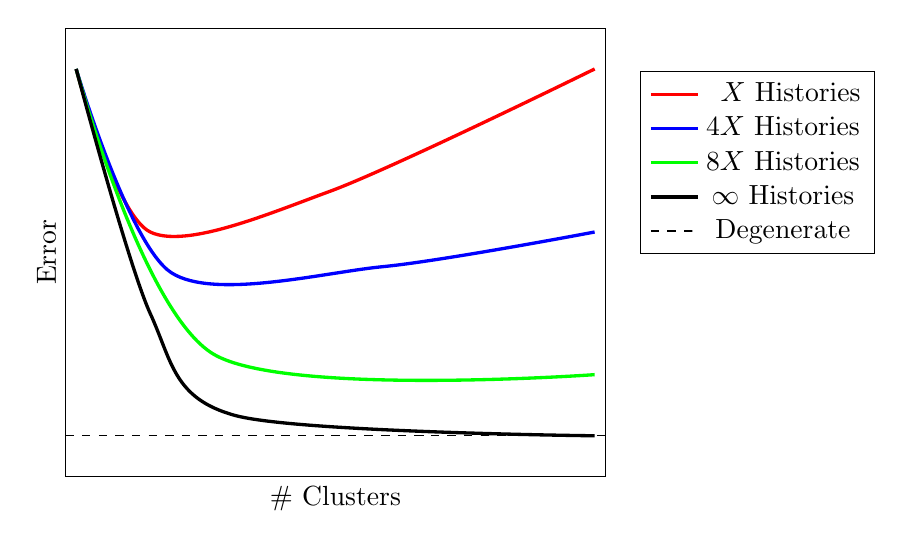
\begin{tikzpicture}
\begin{axis}[xmin=0,xmax=51,ymin=0,ymax=1.1,xlabel={\# Clusters},ylabel={Error},xticklabels={},yticklabels={},xtick={},ytick={},ticks=none,legend style={at={(1.5,0.7)},anchor=east,legend columns=1}]
\addplot[smooth,red,very thick] coordinates { (1,1) (8,0.6) (25,0.7) (50,1) };
\addplot[smooth,blue,very thick] coordinates { (1,1) (10,0.5) (30,0.515) (50,0.6) };
\addplot[smooth,green,very thick] coordinates { (1,1) (14,0.3) (50,0.25) };
\addplot[smooth,very thick] coordinates { (1,1) (8,0.4) (16,0.15) (50,0.1) };
\addplot[smooth,dashed] coordinates { (0,0.1) (51,0.1) };
\addlegendentry{$\;\;X$ Histories}
\addlegendentry{$4X$ Histories}
\addlegendentry{$8X$ Histories}
\addlegendentry{$\infty$ Histories}
\addlegendentry{Degenerate}
\end{axis}
\end{tikzpicture}
\caption[Asympotic convergence of\textit{i}MGXS to degenerate homogenization]{Asymptotic convergence of reaction rate error with \textit{i}\ac{MGXS} in the limit of infinite particle histories to degenerate homogenization with fully converged \ac{MGXS}.}
\label{fig:chap11-coverge-complexity}
\end{figure}

Furthermore, the balance between model complexity and accuracy will depend on the degree of statistical undertainty present in the \ac{MC} tally data, as depicted in Fig.~\ref{fig:chap11-coverge-complexity}. In particular, the statistical uncertainties of the ``noisy'' \ac{MC} tally data for $X$ particle histories will preclude the \textit{i}\ac{MGXS} scheme from achieving the asymptotic accuracy of the degenerate scheme with fully converged \ac{MGXS}. The inclusion of more clusters in \textit{i}\ac{MGXS} scheme will enable it to approach the asymptotic accuracy of the degenerate scheme if enough particle histories have been simulated to reliably estimate the mean of each \ac{MGXS} cluster. The optimal balance between accuracy and speed is achieved when the majority of the gap in accuracy between the null and degenerate schemes is eliminiated with only a few clusters in \textit{i}\ac{MGXS}, which quickly converge with only a fraction of the particle histories needed to converge the \ac{MGXS} for the degenerate scheme.

The maximum and mean errors for \textit{i}\ac{MGXS} with 1 -- 50 clusters are illustrated in Figs.~\Crefrange{fig:chap11-capt-err-by-cluster-assm-16}{fig:capt-err-by-cluster-full-core} for the individual assembly, 2$\times$2 colorset and quarter core \ac{BEAVRS} benchmark models. In particular, the maximum errors are the maximum of the absolute values of the errors, while the mean errors are the averages of the absolute error magnitudes. A couple of key observations can be made with regards to the errors' dependence on the number of clusters, as well as the clustering algorithm. First, it is clear from Figs.~\Crefrange{fig:chap11-capt-err-by-cluster-assm-16}{fig:chap11-capt-err-by-cluster-assm-31-20BPs} that the errors for the individual assemblies is greatly reduced with only 4 -- 8 clusters, with additional clusters having a marginal impact. As expected, the introduction of spatial heterogeneities requires more clusters to converge the error reduction. For example, both the max and mean errors are still trending downward even with 20 clusters for the 2$\times$2 colorset with a water reflector.

%1) the majority of the reduction comes with the inclusion of just a few clusters
%   -max err. for 1.6\% assm (1.1\%) eventually reduces to 0.45\%
%   -just 3 clusters gets to 0.55\%, or 85\% of the reduction with just three clusters
%2) more clusters needed as geometric complexities are added
%   -add BPs
%     -roughly 6 clusters needed for 3.1\% assm, while 10 or so needed with \acp{BP}
%   -add reflector
%     -perioridic colorset mean err saturated with 10 clusters

The different clustering algorithms also vary somewhat in terms of their impact on the max and mean error. However, the figures do not clearly indicate which if any of the algorithms consistently under or overperforms the others for all benchmarks. All four algorithms perform similarly for the 1.6\% and 3.1\% enriched fuel assemblies without \acp{BP} for 1 -- 20 clusters, as shown in Figs.~\Crefrange{fig:chap11-capt-err-by-cluster-assm-16}{fig:chap11-capt-err-by-cluster-assm-31}. Although the mean errors are similar for up to 50 clusters for both assemblies, the max errors fluctuate somewhat erratically between 0.2 -- 0.4\% for 20 -- 50 clusters. Similarly, the mean errors for the 3.1\% enriched assembly with 20 \acp{BP} and the 2$\times$2 colorsets exhibit a consistent downward trend, while the maximum errors separate and fluctuate wildly beyond 10 clusters for the four clustering algorithms. Although no algorithm can be clearly chosen as a ``winner'', \ac{GMM} seems to most consistently outperform the other clustering algorithms for 10 or more clusters. 

Finally, it should be noted that while the mean error is generally a smooth, monotonically decreasing curve, the max error exhibits sharp discontinuities with the addition of clusters. The maximum error likely decreases in a steplike fashion when the addition of a new cluster discriminates those fuel pins with the largest error into their own unique cluster. Evidently, new clusters generally do not refine the \ac{MGXS} for pins with the worst errors. This is likely due to the fact that the $k$-means, agglomerative and \ac{GMM} clustering models optimize a global metric representing the cluster assignments of all points in a dataset, rather than the behavior of the most poorly defined cluster in the model. A revised clustering algorithm may be needed to achieve the maximum error reduction with as few clusters as possible, by successively refining the samples in the most poorly defined clusters. The BIRCH algorithm shows some promise with 10 or fewer clusters, which may be the result of its locally optimized assignment of samples to clusters.

\begin{emphbox}
\textbf{Only a few \ac{MGXS} clusters are needed to substantially reduce the U-238 capture rate errors, with diminishing returns for the inclusion of more clusters. None of the clustering algorithms is a clear winner, though BIRCH generally performs the best for <10 clusters, while \acp{GMM} do better with 10+ clusters.}
\end{emphbox}

%-should mention errors with ICA, PCA, or FA to illustrate that clustering can screw up??? 
%-should mention errors look much different for pinch featur selection???

\begin{figure}[h!]
\centering
\begin{subfigure}{0.9\textwidth}
  \centering
  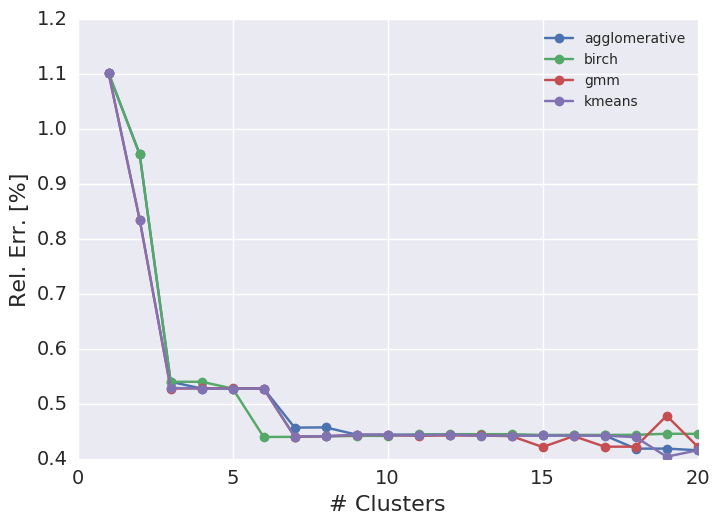
\includegraphics[width=\linewidth]{figures/results/err-by-cluster/assm-16/max-rel-err}
  \caption{}
  \label{fig:chap11-max-capt-err-by-cluster-assm-16}
\end{subfigure}
\begin{subfigure}{0.9\textwidth}
  \centering
  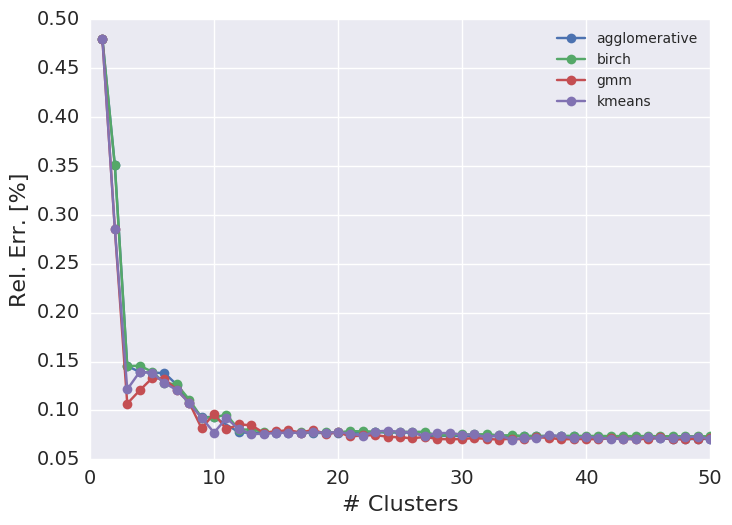
\includegraphics[width=\linewidth]{figures/results/err-by-cluster/assm-16/mean-rel-err}
  \caption{}
  \label{fig:chap11-mean-capt-err-by-cluster-assm-16}
\end{subfigure}
\caption[U-238 capture error for the 1.6\% enriched assembly]{The max (a) and mean (b) U-238 capture rate errors for the 1.6\% enriched assembly with \textit{i}\ac{MGXS} spatial homogenization.}
\label{fig:chap11-capt-err-by-cluster-assm-16}
\end{figure}

\begin{figure}[h!]
\centering
\begin{subfigure}{0.9\textwidth}
  \centering
  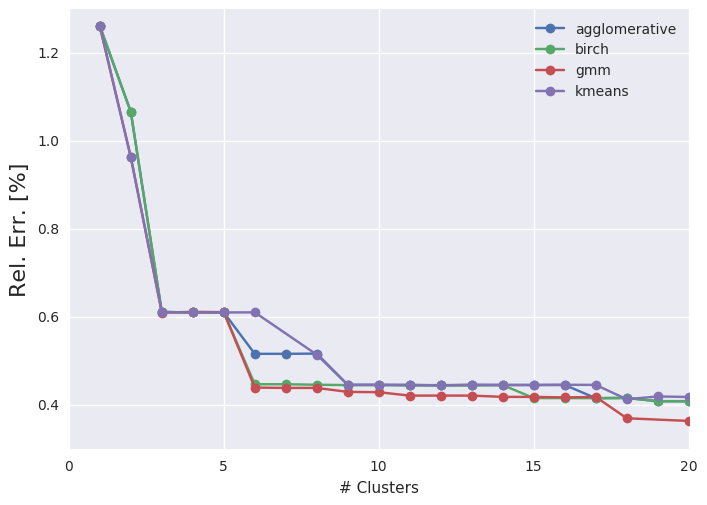
\includegraphics[width=\linewidth]{figures/results/err-by-cluster/assm-31/max-rel-err}
  \caption{}
  \label{fig:chap11-max-capt-err-by-cluster-assm-31}
\end{subfigure}
\begin{subfigure}{0.9\textwidth}
  \centering
  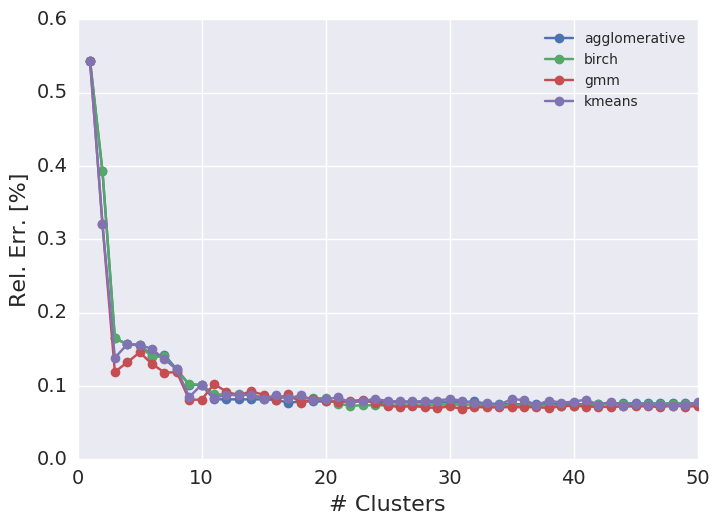
\includegraphics[width=\linewidth]{figures/results/err-by-cluster/assm-31/mean-rel-err}
  \caption{}
  \label{fig:chap11-mean-capt-err-by-cluster-assm-31}
\end{subfigure}
\caption[U-238 capture error for the 3.1\% enriched assembly]{The max (a) and mean (b) U-238 capture rate errors for the 3.1\% enriched assembly with \textit{i}\ac{MGXS} spatial homogenization.}
\label{fig:chap11-capt-err-by-cluster-assm-31}
\end{figure}

\begin{figure}[h!]
\centering
\begin{subfigure}{0.9\textwidth}
  \centering
  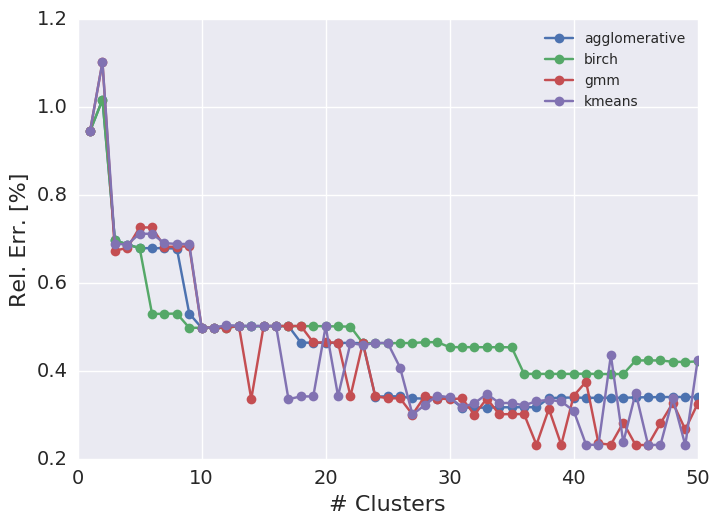
\includegraphics[width=\linewidth]{figures/results/err-by-cluster/assm-31-20BPs/max-rel-err}
  \caption{}
  \label{fig:chap11-max-capt-err-by-cluster-assm-31-20BPs}
\end{subfigure}
\begin{subfigure}{0.9\textwidth}
  \centering
  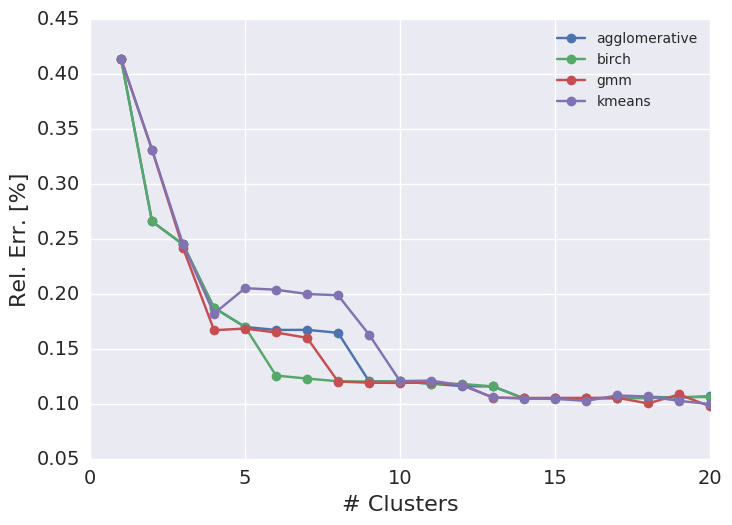
\includegraphics[width=\linewidth]{figures/results/err-by-cluster/assm-31-20BPs/mean-rel-err}
  \caption{}
  \label{fig:chap11-mean-capt-err-by-cluster-assm-31-20BPs}
\end{subfigure}
\caption[U-238 capture error the 3.1\% enriched assembly with 20 BPs]{The max (a) and mean (b) U-238 capture rate errors for the 3.1\% enriched assembly with 20 \acp{BP} with \textit{i}\ac{MGXS} spatial homogenization.}
\label{fig:chap11-capt-err-by-cluster-assm-31-20BPs}
\end{figure}

\begin{figure}[h!]
\centering
\begin{subfigure}{0.9\textwidth}
  \centering
  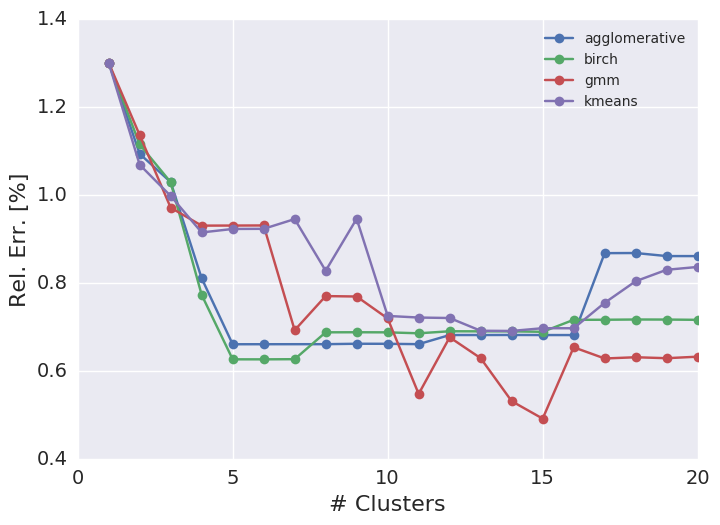
\includegraphics[width=\linewidth]{figures/results/err-by-cluster/2x2/max-rel-err}
  \caption{}
  \label{fig:chap11-max-capt-err-by-cluster-2x2}
\end{subfigure}
\begin{subfigure}{0.9\textwidth}
  \centering
  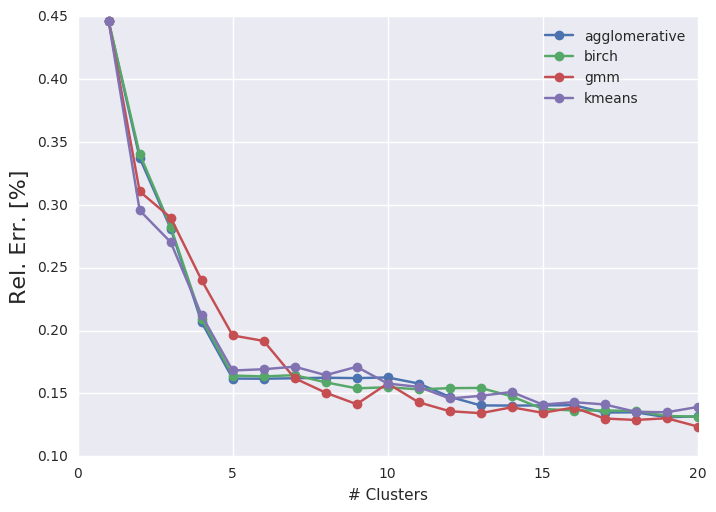
\includegraphics[width=\linewidth]{figures/results/err-by-cluster/2x2/mean-rel-err}
  \caption{}
  \label{fig:chap11-mean-capt-err-by-cluster-2x2}
\end{subfigure}
\caption[U-238 capture error for the 2$\times$2 colorset]{The max (a) and mean (b) U-238 capture rate error for the 2$\times$2 colorset with \textit{i}\ac{MGXS} spatial homogenization.}
\label{fig:chap11-capt-err-by-cluster-2x2}
\end{figure}

\begin{figure}[h!]
\centering
\begin{subfigure}{0.9\textwidth}
  \centering
  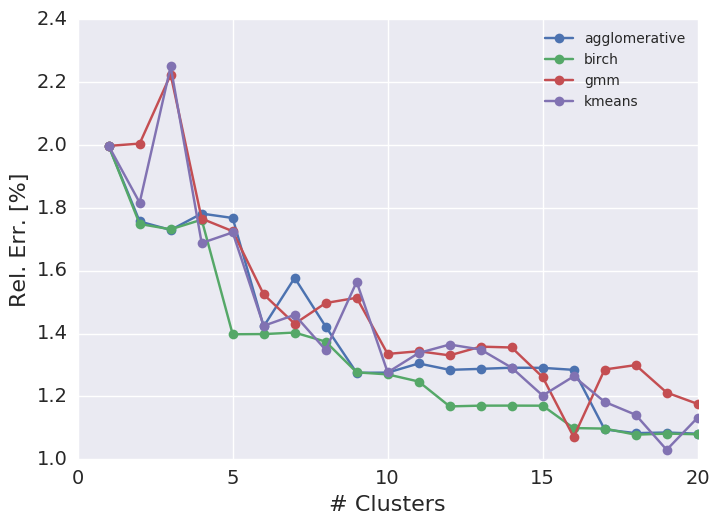
\includegraphics[width=\linewidth]{figures/results/err-by-cluster/reflector/max-rel-err}
  \caption{}
  \label{fig:chap11-max-capt-err-by-cluster-refl}
\end{subfigure}
\begin{subfigure}{0.9\textwidth}
  \centering
  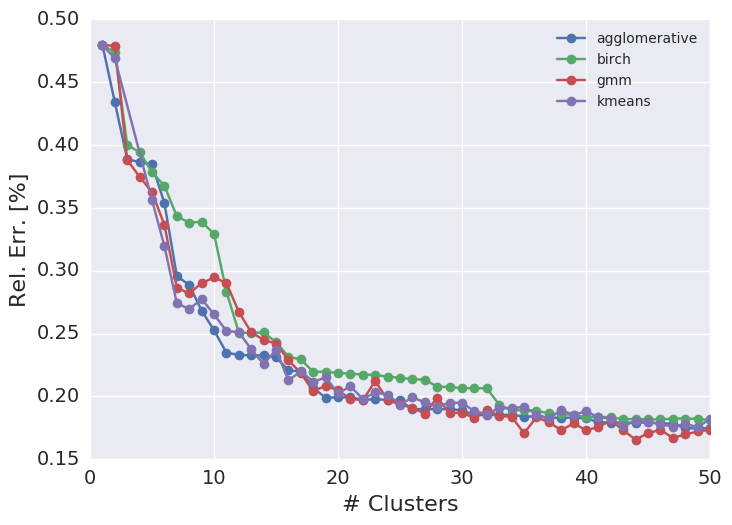
\includegraphics[width=\linewidth]{figures/results/err-by-cluster/reflector/mean-rel-err}
  \caption{}
  \label{fig:chap11-mean-capt-err-by-cluster-refl}
\end{subfigure}
\caption[U-238 capture error for the 2$\times$2 colorset with reflector]{The max (a) and mean (b) U-238 capture rate error for the 2$\times$2 colorset with water reflector with \textit{i}\ac{MGXS} spatial homogenization.}
\label{fig:chap11-capt-err-by-cluster-refl}
\end{figure}

\begin{figure}[h!]
\centering
\begin{subfigure}{0.9\textwidth}
  \centering
  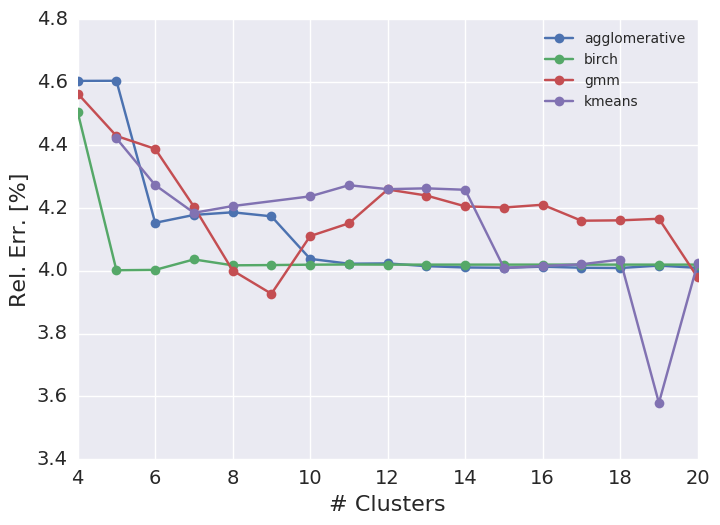
\includegraphics[width=\linewidth]{figures/results/err-by-cluster/full-core/max-rel-err}
  \caption{}
  \label{fig:max-capt-err-by-cluster-full-core}
\end{subfigure}
\begin{subfigure}{0.9\textwidth}
  \centering
  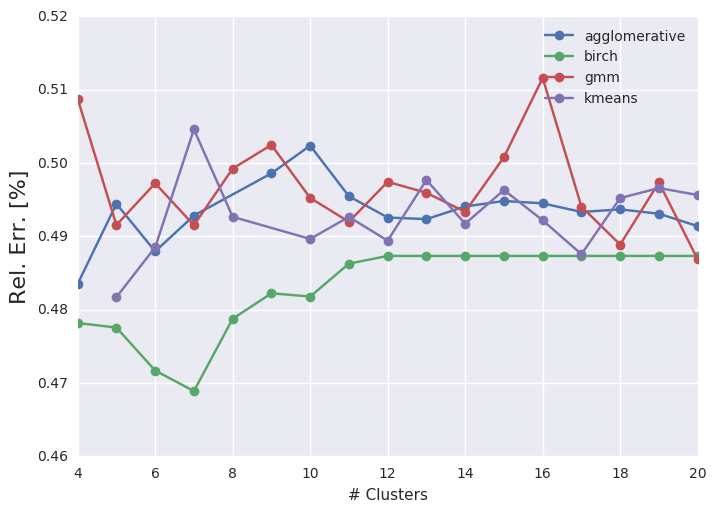
\includegraphics[width=\linewidth]{figures/results/err-by-cluster/full-core/mean-rel-err}
  \caption{}
  \label{fig:mean-capt-err-by-cluster-full-core}
\end{subfigure}
\caption[U-238 capture error for quarter core BEAVRS model]{The max (a) and mean (b) U-238 capture rate error for the quarter core \ac{BEAVRS} model with \textit{i}\ac{MGXS} spatial homogenization.}
\label{fig:capt-err-by-cluster-full-core}
\end{figure}

\clearpage

%%%%%%%%%%%%%%%%%%%%%%%%%%%%%%%%%%%%%%%%%%%%%%%%%%%%%%%%%%%%%%
\subsubsection{Benchmark with Null and Degenerate Schemes}
\label{subsec:chap11-imgxs-capt-rates-benchmark}

The maximum and mean percent relative errors for each pin's U-238 capture rates are listed for each benchmark in Tabs.~\ref{table:chap11-max-capt-rates} and~\ref{table:chap11-mean-capt-rates}, respectively, for a variable number of clusters for each clustering algorithm. In particular, the maximum errors are the maximum of the absolute values of the errors along with the appropriate sign, while the mean errors are the averages of the absolute error magnitudes. The errors are tabulated for 2 -- 16 clusters, along with null homogenization (one cluster for all pin instances) and degenerate homogenization (one cluster per pin instance).

Since the tables simply represent a snapshot of the data illustrated in Figs.~\Crefrange{fig:chap11-capt-err-by-cluster-assm-16}{fig:capt-err-by-cluster-full-core}, the observations made in Sec.~\ref{subsec:chap11-imgxs-capt-rates-num-clusters} remain valid here. First, the majority of the error is reduced with only a few clusters. For example, 70 -- 80\% of the reduction in the maximum error enabled with degenerate homogenization can be achieved with only 4 clusters for the 1.6\% and 3.1\% enriched fuel assembly benchmarks without \acp{BP}. Although 16 clusters (or more) are needed to reduce the error to 70\% for the 3.1\% enriched assembly with 20 \acp{BP}, over 75\% of the error reduction is achieved with only 4 clusters for the periodic 2$\times$2 colorset. Likewise, the addition of a water reflector to the colorset necessitates the use of 16 or more clusters to reduce the error by 75\% or more. In addition, the maximum errors exhibit greater variation across algorithms than the mean errors, as was previously noted in Sec.~\ref{subsec:chap11-imgxs-capt-rates-num-clusters}. Finally, the BIRCH and \ac{GMM} algorithms generally achieve smaller errors than the $k$-means and agglomerative clustering algorithms for a fixed number of clusters.

\begin{table}[h!]
  \centering
  \caption[Maximum OpenMOC U-238 capture rate errors]{Maximum absolute U-238 capture rate percent relative errors for \textit{i}\ac{MGXS} spatial homogenization for each clustering algorithm.}
  \small
  \label{table:chap11-max-capt-rates}
  \vspace{6pt}
  \begin{tabular}{l l R{1.2cm} R{1.2cm} R{1.2cm} R{1.2cm} R{1.2cm} R{1.2cm}}
  \toprule
  \rowcolor{lightgray}
  & \multicolumn{1}{c}{\cellcolor{lightgray} \bf Clustering} & \multicolumn{6}{S[table-format=6.1]}{\cellcolor{lightgray} \textbf{\# Clusters}} \\
  \multirow{-2}{*}{\cellcolor{lightgray} \bf Benchmark} &
  \multicolumn{1}{c}{\cellcolor{lightgray} \bf Algorithm} &
  \multicolumn{1}{c}{\cellcolor{lightgray} \bf 1\textsuperscript{\ref{null}}} &
  \multicolumn{1}{c}{\cellcolor{lightgray} \bf 2} &
  \multicolumn{1}{c}{\cellcolor{lightgray} \bf 4} &
  \multicolumn{1}{c}{\cellcolor{lightgray} \bf 8} &
  \multicolumn{1}{c}{\cellcolor{lightgray} \bf 16} &
  \multicolumn{1}{c}{\cellcolor{lightgray} \bf \# pins\textsuperscript{\ref{degenerate}}} \\
  \midrule
\multirow{4}{*}{\parbox{2.5cm}{1.6\% Assm}} & Agglomerative & \multirow{4}{*}{-1.10} & 0.95 & -0.53 & -0.46 & -0.44 & \multirow{4}{*}{0.38} \\
& BIRCH & & 0.95 & -0.54 & -0.44 & -0.44 & \\
& \ac{GMM} & & -0.84 & -0.53 & -0.44 & -0.44 & \\
& $k$-means & & -0.84 & -0.53 & -0.44 & -0.44 & \\
  \midrule
\multirow{4}{*}{\parbox{2.5cm}{3.1\% Assm}} & Agglomerative & \multirow{4}{*}{-1.26} & 1.07 & -0.61 & -0.52 & 0.45 & \multirow{4}{*}{-0.33} \\
& BIRCH & & 1.07 & -0.61 & 0.45 & -0.42 & \\
& \ac{GMM} & & -0.96 & -0.61 & -0.44 & -0.42 & \\
& $k$-means & & -0.96 & -0.61 & -0.52 & 0.45 & \\
  \midrule
\multirow{4}{*}{\parbox{2.5cm}{3.1\% Assm w/ 20 BPs}} & Agglomerative & \multirow{4}{*}{-0.95} & -1.02 & 0.69 & 0.68 & -0.50 & \multirow{4}{*}{-0.30} \\
& BIRCH & & -1.02 & 0.69 & -0.53 & -0.50 & \\
& \ac{GMM} & & -1.10 & 0.68 & -0.53 & -0.50 & \\
& $k$-means & & -1.10 & 0.69 & -0.69 & 0.34 & \\
  \midrule
\multirow{4}{*}{\parbox{2.5cm}{2$\times$2 Colorset}} & Agglomerative & \multirow{4}{*}{-1.30} & -1.09 & 0.81 & 0.66 & 0.68 & \multirow{4}{*}{-0.64} \\
& BIRCH & & -1.12 & 0.77 & 0.69 & 0.72 & \\
& \ac{GMM} & & -1.14 & 0.93 & 0.77 & 0.65 & \\
& $k$-means & & -1.07 & -0.92 & -0.83 & 0.70 & \\
  \midrule
\multirow{4}{*}{\parbox{2.5cm}{2$\times$2 Colorset w/ Reflector}} & Agglomerative & \multirow{4}{*}{-2.00} & -1.76 & -1.78 & -1.42 & -1.28 & \multirow{4}{*}{-0.80} \\
& BIRCH & & -1.75 & -1.76 & -1.37 & 1.10 & \\
& \ac{GMM} & & -2.00 & -1.77 & 1.50 & 1.07 & \\
& $k$-means & & -1.82 & -1.69 & 1.35 & -1.26 & \\
  \midrule
\multirow{4}{*}{\parbox{2.5cm}{BEAVRS Full Core}} & Agglomerative & \multirow{4}{*}{-4.78} & & -4.60 & -4.19 & -4.01 & \multirow{4}{*}{-3.03} \\
& BIRCH & & & -4.51 & -4.02 & -4.02 & \\
& \ac{GMM} & & & -4.56 & -4.00 & -4.21 & \\
& $k$-means & & & -4.61 & -4.21 & -4.02 & \\
  \bottomrule
\end{tabular}
\end{table}

\clearpage

\begin{table}[h!]
  \centering
  \caption[Mean OpenMOC U-238 capture rate errors]{Mean absolute U-238 capture rate percent relative errors for \textit{i}\ac{MGXS} spatial homogenization for each clustering algorithm.}
  \small
  \label{table:chap11-mean-capt-rates}
  \vspace{6pt}
  \begin{tabular}{l l R{1.2cm} R{1.2cm} R{1.2cm} R{1.2cm} R{1.2cm} R{1.2cm}}
  \toprule
  \rowcolor{lightgray}
  & \multicolumn{1}{c}{\cellcolor{lightgray} \bf Clustering} & \multicolumn{6}{S[table-format=6.1]}{\cellcolor{lightgray} \textbf{\# Clusters}} \\
  \multirow{-2}{*}{\cellcolor{lightgray} \bf Benchmark} &
  \multicolumn{1}{c}{\cellcolor{lightgray} \bf Algorithm} &
  \multicolumn{1}{c}{\cellcolor{lightgray} \bf 1\textsuperscript{\ref{null}}} &
  \multicolumn{1}{c}{\cellcolor{lightgray} \bf 2} &
  \multicolumn{1}{c}{\cellcolor{lightgray} \bf 4} &
  \multicolumn{1}{c}{\cellcolor{lightgray} \bf 8} &
  \multicolumn{1}{c}{\cellcolor{lightgray} \bf 16} &
  \multicolumn{1}{c}{\cellcolor{lightgray} \bf \# pins\textsuperscript{\ref{degenerate}}} \\
  \midrule
\multirow{4}{*}{\parbox{2.5cm}{1.6\% Assm}} & Agglomerative & \multirow{4}{*}{0.48} & 0.35 & 0.14 & 0.11 & 0.08 & \multirow{4}{*}{0.08} \\
& BIRCH & & 0.35 & 0.15 & 0.11 & 0.08 & \\
& \ac{GMM} & & 0.29 & 0.12 & 0.11 & 0.08 & \\
& $k$-means & & 0.29 & 0.14 & 0.11 & 0.08 & \\
  \midrule
\multirow{4}{*}{\parbox{2.5cm}{3.1\% Assm}} & Agglomerative & \multirow{4}{*}{0.54} & 0.39 & 0.16 & 0.12 & 0.08 & \multirow{4}{*}{0.09} \\
& BIRCH & & 0.39 & 0.16 & 0.12 & 0.08 \\
& \ac{GMM} & & 0.32 & 0.13 & 0.10 & 0.09 & \\
& $k$-means & & 0.32 & 0.16 & 0.12 & 0.09 & \\
  \midrule
\multirow{4}{*}{\parbox{2.5cm}{3.1\% Assm w/ 20 BPs}} & Agglomerative & \multirow{4}{*}{0.41} & 0.27 & 0.19 & 0.17 & 0.11 & \multirow{4}{*}{0.09} \\
& BIRCH & & 0.27 & 0.19 & 0.12 & 0.11 & \\
& \ac{GMM} & & 0.33 & 0.17 & 0.12 & 0.11 & \\
& $k$-means & & 0.33 & 0.18 & 0.20 & 0.10 & \\
  \midrule
\multirow{4}{*}{\parbox{2.5cm}{2$\times$2 Colorset}} & Agglomerative & \multirow{4}{*}{0.45} & 0.34 & 0.21 & 0.16 & 0.14 & \multirow{4}{*}{0.15} \\
& BIRCH & & 0.34 & 0.21 & 0.16 & 0.14 & \\
& \ac{GMM} & & 0.31 & 0.24 & 0.15 & 0.14 & \\
& $k$-means & & 0.30 & 0.21 & 0.16 & 0.14 & \\
  \midrule
\multirow{4}{*}{\parbox{2.5cm}{2$\times$2 Colorset w/ Reflector}} & Agglomerative & \multirow{4}{*}{0.48} & 0.43 & 0.39 & 0.29 & 0.22 & \multirow{4}{*}{0.16} \\
& BIRCH & & 0.47 & 0.39 & 0.34 & 0.23 & \\
& \ac{GMM} & & 0.48 & 0.37 & 0.29 & 0.24 & \\
& $k$-means & & 0.47 & 0.37 & 0.27 & 0.22 & \\
  \midrule
\multirow{4}{*}{\parbox{2.5cm}{BEAVRS Full Core}} & Agglomerative & \multirow{4}{*}{0.49} & & 0.48 & 0.49 & 0.49 & \multirow{4}{*}{0.39} \\
& BIRCH & & & 0.48 & 0.48 & 0.49 & \\
& \ac{GMM} & & & 0.51 & 0.50 & 0.51 & \\
& $k$-means & & & 0.50 & 0.49 & 0.49 & \\
  \bottomrule
\end{tabular}
\end{table}

\clearpage

%%%%%%%%%%%%%%%%%%%%%%%%%%%%%%%%%%%%%%%%%%%%%%%%%%%%%%%%%%%%%%%%%%
\subsubsection{Spatial Distributions of U-238 Capture Rate Errors}
\label{subsec:chap11-imgxs-capt-rates-space-distrib}

The spatial distributions of capture rate errors are plotted as heatmaps for the assembly and colorset benchmarks in Figs.~\Crefrange{fig:chap11-assm-1.6-capt-err}{fig:chap11-refl-capt-err} with null, degenerate, \ac{LNS} and \textit{i}\ac{MGXS} homogenization with BIRCH clustering of 2, 4 and 16 clusters. The capture rate errors for the full core are illustrated in Fig.~\ref{fig:chap11-full-core-capt-err-a} for null and degenerate homogenization, and in Fig.~\ref{fig:chap11-full-core-capt-err-b} for \textit{i}\ac{MGXS} homogenization with BIRCH clustering of 4 and 16 clusters.

A couple of key conclusions can be drawn from these results. First, the results from Sec.~\ref{subsec:chap11-imgxs-capt-rates-benchmark} indicated that the errors with \textit{i}\ac{MGXS} homogenization with 16 clusters exceed those for degenerate homogenization for both the 3.1\% enriched fuel assembly with 20 \acp{BP} and the periodic 2$\times$2 colorset. This is revealed in the Figs.~\Crefrange{fig:chap11-assm-3.1-20BPs-capt-err}{fig:chap11-2x2-capt-err} which illustrate a systematic bias which differs from that of the degenerate case. In particular, those pins which are facially and diagonally adjacent to the central instrument tube exhibit the smallest and largest errors in the assembly with 20 \acp{BP}, respectively. Likewise, the pins between the two rings of \acp{BP} in the 3.1\% enriched fuel assembly exhibit the largest errors for the periodic colorset. These observations are particularly interesting since the \ac{LNS} scheme outperforms \textit{i}\ac{MGXS} for these benchmarks while using substantially fewer materials (9 -- 10 \ac{LNS} materials as compared to 16 \textit{i}\ac{MGXS} materials per assembly). Although \ac{LNS} necessarily discriminates those pins adjacent to the instrument tube and \acp{BP} into unique clusters, the \textit{i}\ac{MGXS} scheme only does so if the feature vectors for those fuel pins are well-separated from those for other fuel pins in feature space.

Unlike the \ac{LNS} scheme, the \textit{i}\ac{MGXS} scheme excels at discriminating pins along assembly-assembly and assembly-reflector interfaces as shown in Figs.~\Crefrange{fig:chap11-2x2-capt-err}{fig:chap11-refl-capt-err}\footnote{However, even with 16 clusters, there are some lingering residual errors for pins along the interfaces between the bottom right assembly and its neighbors.}. This is most obvious for the pins along the assembly-reflector interface which exhibit nearly the same error for both null and \ac{LNS} homogenization. The \textit{i}\ac{MGXS} scheme discriminates these pins into unique clusters such that little if any residual bias is observed with 16 clusters. Indeed, the \textit{i}\ac{MGXS} scheme dedicates unique clusters to those pins along the interfaces \textit{before} discriminating interior pins adjacent to \acp{CRGT} and \acp{BP} into clusters. For this reason, \textit{i}\ac{MGXS} may necessarily need to model more unique materials than \ac{LNS} to achieve the same reduction in the maximum pin-wise error.

Finally, it should be noted that the observations made here are specific to the configuration of the \textit{i}\ac{MGXS} data processing pipeline. In particular, each of the figures for \textit{i}\ac{MGXS} spatial homogenization corresponds to a prediction by the BIRCH clustering algorithm with litmus-only feature selection. As noted in Sec.~\ref{sec:chap10-cluster-geometries}, the choice of features and clustering algorithm has a large impact on the clustering model and the resultant spatial distribution of U-238 capture rate errors. In addition, dimensionality reduction adds another degree of freedom to the types of clustered geometries that may be found with the \textit{i}\ac{MGXS} scheme. Future work should systematically examine the spatial error distributions for different configurations of the \textit{i}\ac{MGXS} data processing pipeline to quantify the ability of each minimize error with as few clusters as possible.

\begin{emphbox}
\textbf{The \textit{i}\ac{MGXS} scheme does a better job discriminating fuel pins along assembly-assembly and assembly-reflector interfaces than \ac{LNS}, but requires more unique materials to achieve the same reduction in U-238 capture rate errors.}
\end{emphbox}

%-note that \ac{LNS} did better than degenerate for each benchmark except for reflected colorset

\begin{figure}[h!]
\centering
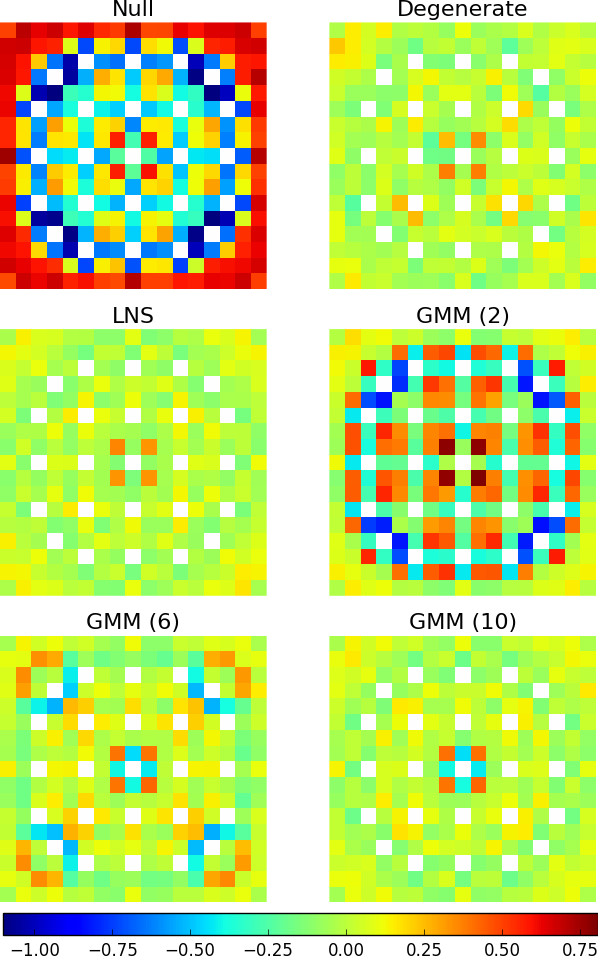
\includegraphics[width=0.87\linewidth]{figures/results/spatial/assm-16/capt-err}
\vspace{2mm}
\caption[U-238 capture errors for the 1.6\% enriched assembly]{U-238 capture percent relative errors for the 1.6\% enriched assembly with null, degenerate, \ac{LNS} and \textit{i}\ac{MGXS} spatial homogenization.}
\label{fig:chap11-assm-1.6-capt-err}
\end{figure}

\clearpage

\begin{figure}[h!]
\centering
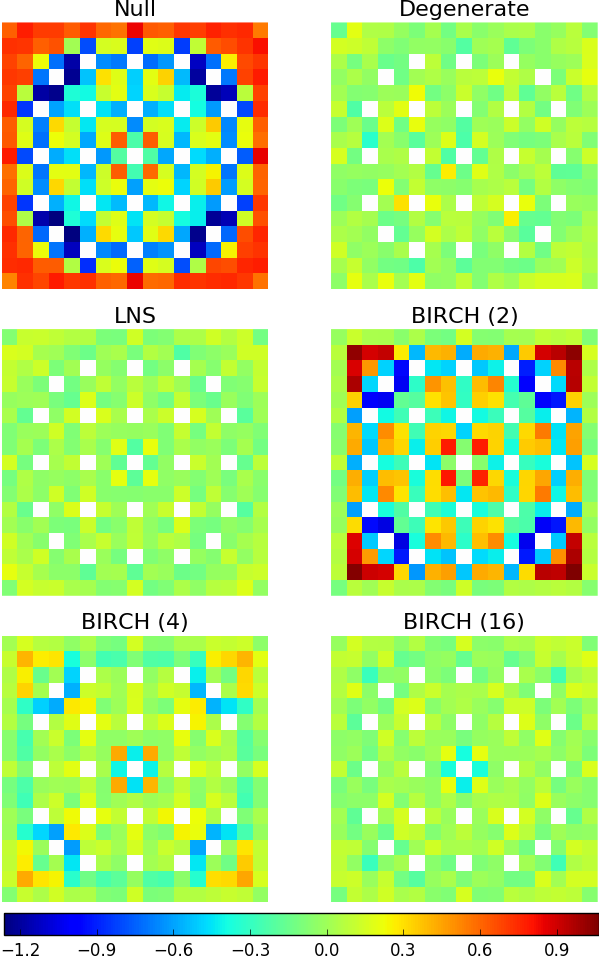
\includegraphics[width=0.87\linewidth]{figures/results/spatial/assm-31/capt-err}
\vspace{2mm}
\caption[U-238 capture errors for the 3.1\% enriched assembly]{U-238 capture percent relative errors for the 3.1\% enriched assembly with null, degenerate, \ac{LNS} and \textit{i}\ac{MGXS} spatial homogenization.}
\label{fig:chap11-assm-3.1-capt-err}
\end{figure}

\clearpage

\begin{figure}[h!]
\centering
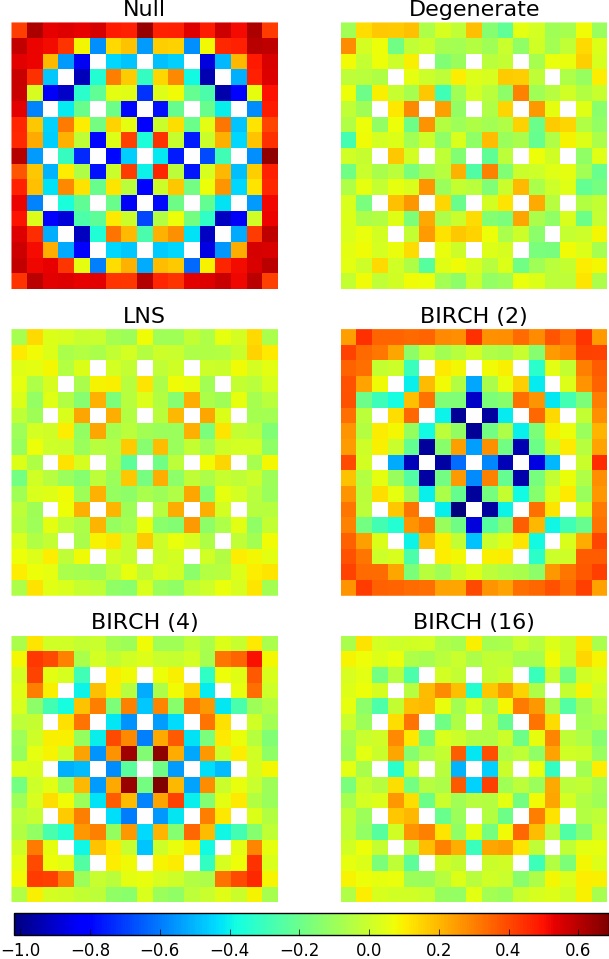
\includegraphics[width=0.87\linewidth]{figures/results/spatial/assm-31-20BPs/capt-err}
\vspace{2mm}
\caption[U-238 capture errors for the 3.1\% enriched assembly with 20 BPs]{U-238 capture percent relative errors for the 3.1\% enriched assembly with 20 \acp{BP} with null, degenerate, \ac{LNS} and \textit{i}\ac{MGXS} spatial homogenization.}
\label{fig:chap11-assm-3.1-20BPs-capt-err}
\end{figure}

\clearpage

\begin{figure}[h!]
\centering
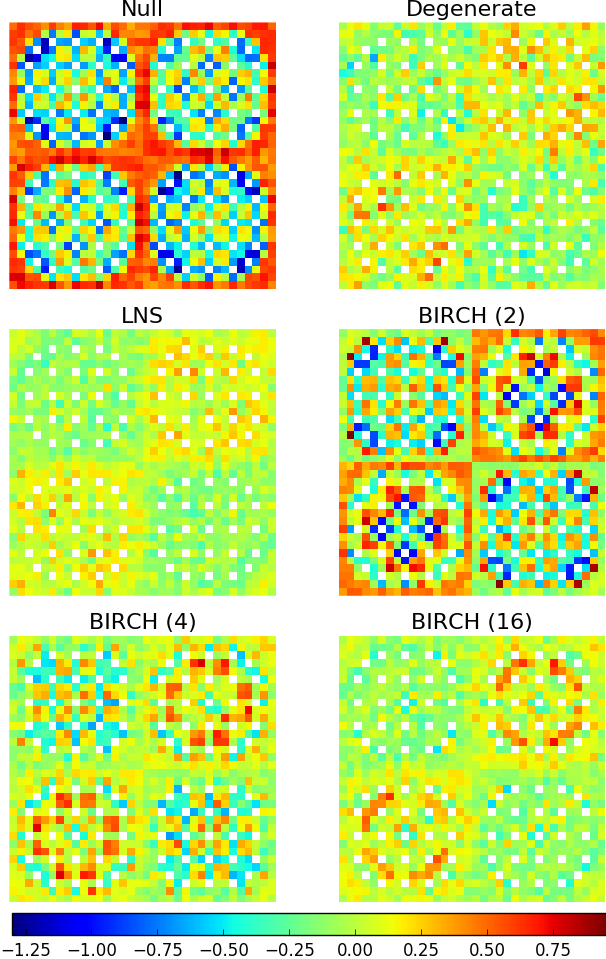
\includegraphics[width=0.87\linewidth]{figures/results/spatial/2x2/capt-err}
\vspace{2mm}
\caption[U-238 capture errors for the 2$\times$2 colorset]{U-238 capture percent relative errors for the 2$\times$2 colorset with null, degenerate, \ac{LNS} and \textit{i}\ac{MGXS} spatial homogenization.}
\label{fig:chap11-2x2-capt-err}
\end{figure}

\clearpage

\begin{figure}[h!]
\centering
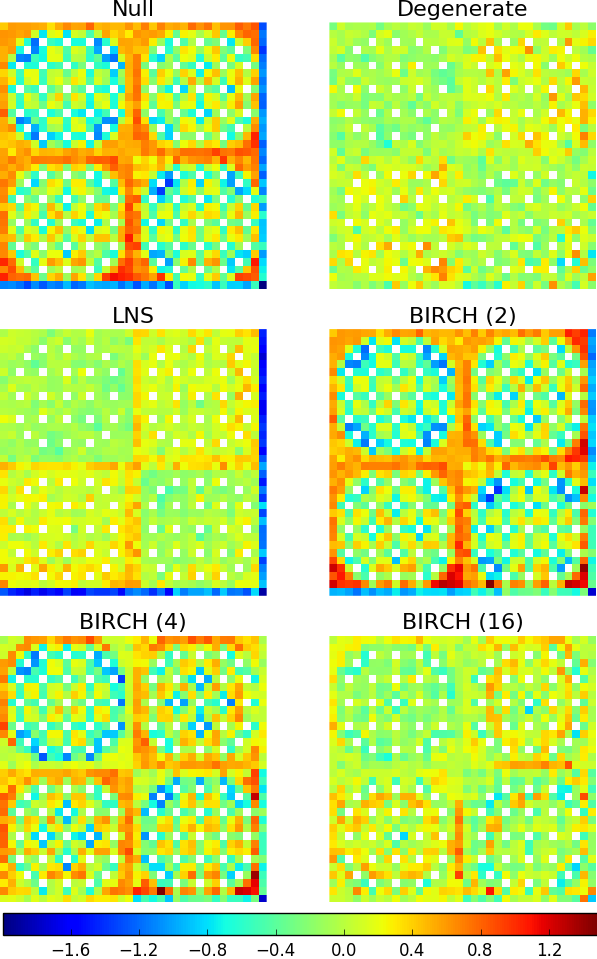
\includegraphics[width=0.87\linewidth]{figures/results/spatial/reflector/capt-err}
\vspace{2mm}
\caption[U-238 capture errors for the 2$\times$2 colorset with reflector]{U-238 capture percent relative errors for the 2$\times$2 colorset with a water reflector with null, degenerate, \ac{LNS} and \textit{i}\ac{MGXS} spatial homogenization.}
\label{fig:chap11-refl-capt-err}
\end{figure}

\clearpage

\begin{figure}[h!]
\centering
\begin{subfigure}{0.9\textwidth}
  \centering
  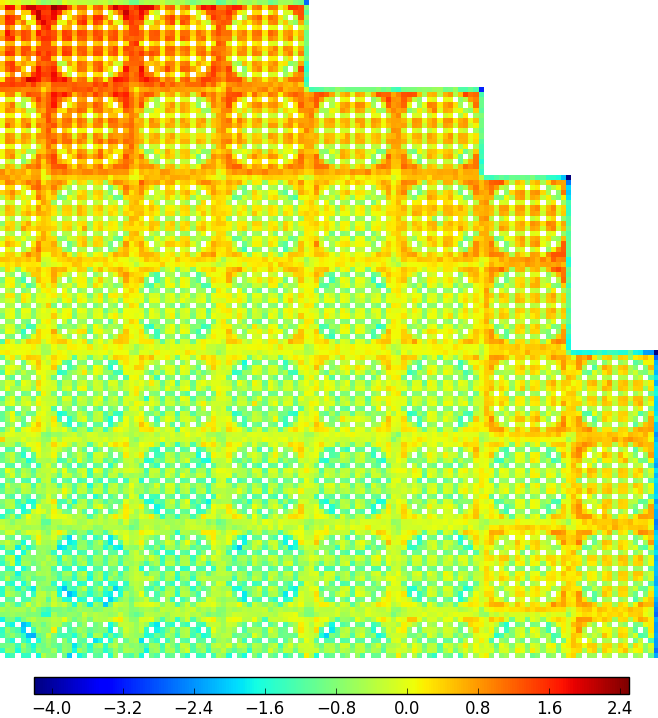
\includegraphics[width=0.65\linewidth]{figures/results/spatial/full-core/capt-err-null}
  \caption{}
  \label{fig:chap11-full-core-capt-err-null}
\end{subfigure}
\begin{subfigure}{0.9\textwidth}
  \centering
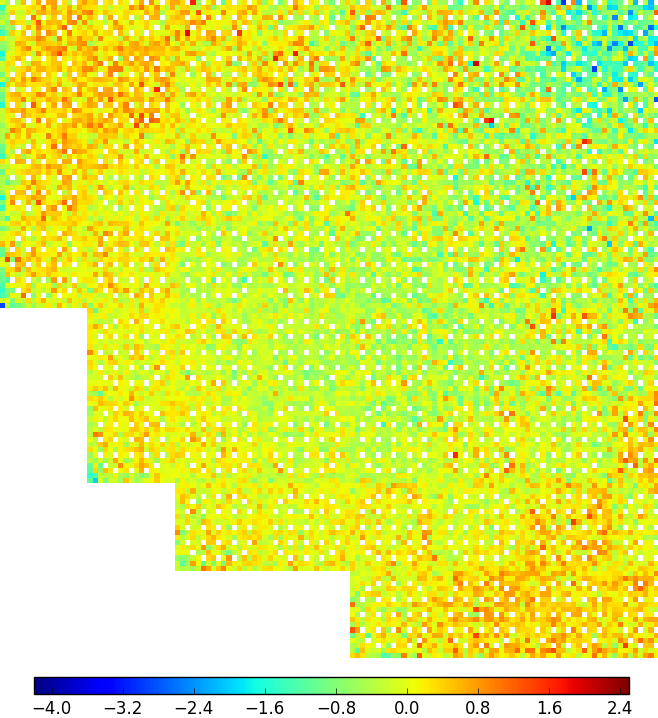
\includegraphics[width=0.65\linewidth]{figures/results/spatial/full-core/capt-err-degenerate}
  \caption{}
  \label{fig:chap11-full-core-capt-err-degenerate}
\end{subfigure}
\caption[U-238 capture rate errors for \ac{BEAVRS}]{U-238 capture percent relative errors for the quarter core \ac{BEAVRS} model with null (a) and degenerate (b) spatial homogenization.}
\label{fig:chap11-full-core-capt-err-a}
\end{figure}

\clearpage

\begin{figure}[h!]
\centering
\begin{subfigure}{0.9\textwidth}
  \centering
  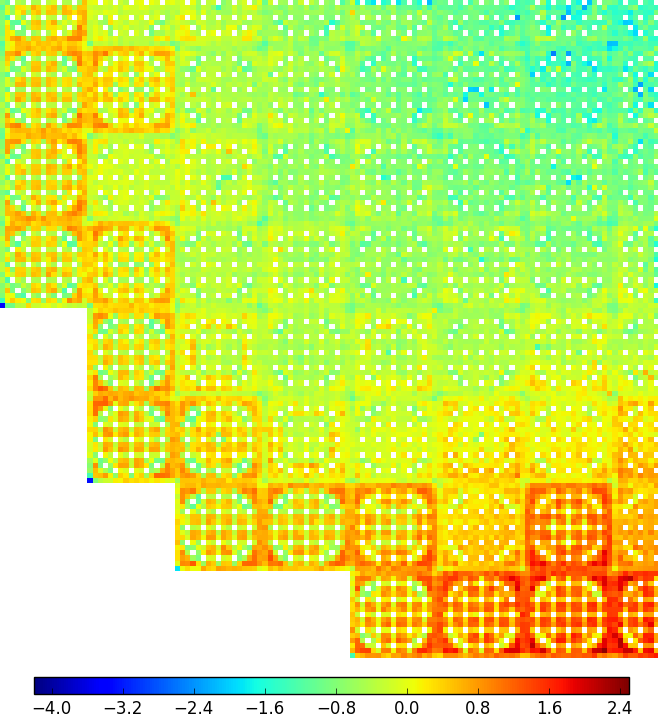
\includegraphics[width=0.65\linewidth]{figures/results/spatial/full-core/capt-err-birch-4}
  \caption{}
  \label{fig:chap11-full-core-capt-err-birch-4}
\end{subfigure}
\begin{subfigure}{0.9\textwidth}
  \centering
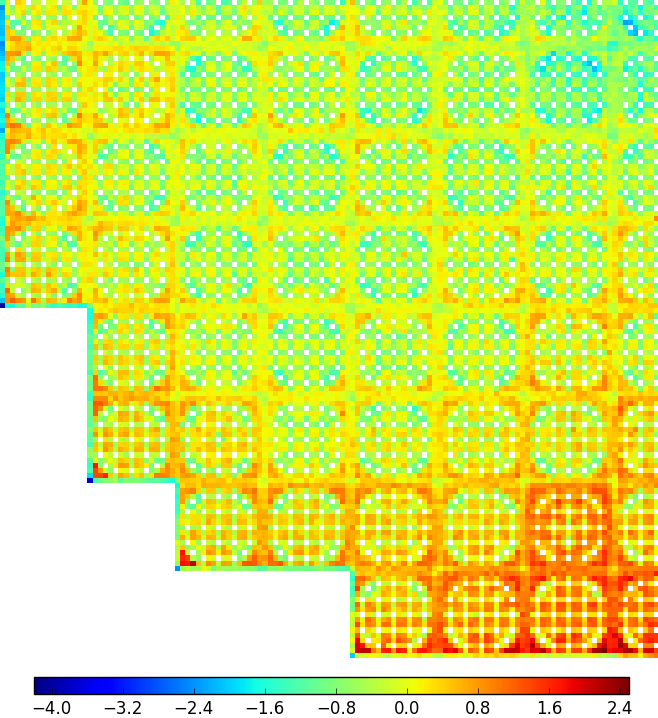
\includegraphics[width=0.65\linewidth]{figures/results/spatial/full-core/capt-err-birch-16}
  \caption{}
  \label{fig:chap11-full-core-capt-err-birch-16}
\end{subfigure}
\caption[U-238 capture rate errors for \ac{BEAVRS}]{U-238 capture percent relative errors for the quarter core \ac{BEAVRS} model with \textit{i}\ac{MGXS} spatial homogenization with BIRCH clustering of 4 (a) and 16 (b) clusters.}
\label{fig:chap11-full-core-capt-err-b}
\end{figure}

\clearpage

%%%%%%%%%%%%%%%%%%%%%%%%%%%%%%%%%%%%%%%%%%%
\subsubsection{Comparing OpenMOC Solutions}
\label{subsec:chap11-imgxs-capt-rates-compare}

This section directly compares the reaction rates from two different OpenMOC simulations with null and \textit{i}\ac{MGXS} homogenization to better understand the impact of \ac{MGXS} clustering on the spatial distribution of U-238 capture rate errors. In particular, the percent relative deviation $\Delta_{k}^{\mathrm{\textit{i}MGXS}}$ of the OpenMOC U-238 capture rate distributions between the null and \textit{i}\ac{MGXS} schemes is computed as follows:

\begin{equation}
\label{eqn:chap11-compare-openmoc}
\Delta_{k}^{\mathrm{\textit{i}MGXS}} \;\; [\%] \;\; = \;\; \frac{\displaystyle\sum\limits_{g=1}^{G} \hat{\Sigma}^{238}_{\gamma,k,g}\phi_{k,g}^{\mathrm{\textit{i}MGXS}} - \displaystyle\sum\limits_{g=1}^{G} \hat{\Sigma}^{238}_{\gamma,k,g}\phi_{k,g}^{\mathrm{Null}}}{\displaystyle\sum\limits_{g=1}^{G} \hat{\Sigma}^{238}_{\gamma,k,g}\phi_{k,g}^{\mathrm{Null}}} \times 100
\end{equation}

\noindent Unlike the U-238 capture rate error distributions, the relative deviations are not sensitive to the statistical uncertainties of the OpenMC reference solutions. As a result, it is easier to easier to visualize the impact of clusters on the U-238 capture rate predictions. Figs.~\Crefrange{fig:chap11-assm-1.6-capt-rates-comp}{fig:chap11-refl-capt-rates-comp} present the percent relative deviations for the individual assembly and 2$\times$2 colorset benchmarks for BIRCH clustering of 2, 4, 8 and 16 clusters. Likewise, Figs.~\Crefrange{fig:chap11-full-core-capt-rates-kmeans-comp}{fig:chap11-full-core-capt-rates-birch-comp} illustrate the deviations for the quarter core \ac{BEAVRS} model with $k$-means, \ac{GMM} and BIRCH clustering of 4, 8, 16 and 20 clusters, respectively.

The figures illustrate the hierarchical nature of \ac{MGXS} clustering by discriminating fuel pins with different spatial self-shielding effects that occur in different regimes. For example, the first 2 clusters used for the individual assemblies distinguishes fuel pins which are adjacent (or nearly adjacent) to \acp{CRGT}, \acp{BP} or instrument tubes from those which are only surrounded by other fuel pins. The introduction of more clusters further refines these clusters to identify fuel pins with neighbors which induce similar spatial self-shielding effects. Of particular note, as the \textit{i}\ac{MGXS} scheme transitions between 8 -- 16 clusters for the 3.1\% enriched fuel assembly with 20 \acp{BP} (Fig.~\ref{fig:chap11-assm-31-20BPs-capt-rates-comp}), the fuel pins that are facially and diagonally adjacent to two \acp{CRGT} are separated into their own cluster. As a result, these eight fuel pins have the largest relative deviation from null homogenization since they experience the largest amount of differential moderation from the two \acp{CRGT}. Similarly, the first 2 -- 4 clusters in the colorset with a reflector (Fig.~\ref{fig:chap11-refl-capt-rates-comp}) discriminate pins along the assembly-assembly and assembly-reflector interfaces. As more clusters are introduced, they are increasingly customized to model the more local spatial self-shielding effects affecting the pins within the interior of each assembly due to the presence of \acp{CRGT} and \acp{BP}.

As was noted in Sec.~\ref{subsec:chap11-imgxs-capt-rates-space-distrib}, the observations made here are specific to the configuration of the \textit{i}\ac{MGXS} data processing pipeline. The choice of features, dimensionality reduction technique(s) and clustering algorithm has a large impact on the clustering model and the resultant spatial distribution of U-238 capture rate errors, and should be further investigated in the future.

\begin{emphbox}
\textbf{The percent relative deviations between OpenMOC solutions with null and \textit{i}\ac{MGXS} homogenization makes it easy to discern the hierarchical nature of \ac{MGXS} clustering and its impact on U-238 capture rate predictions.}
\end{emphbox}

% than is possible with spatial distributions of errors with respect to a ``noisy'' Monte Carlo reference solution.

%-note a few outlier pins in the periodic colorset which break the symmetry

\begin{figure}[h!]
\centering
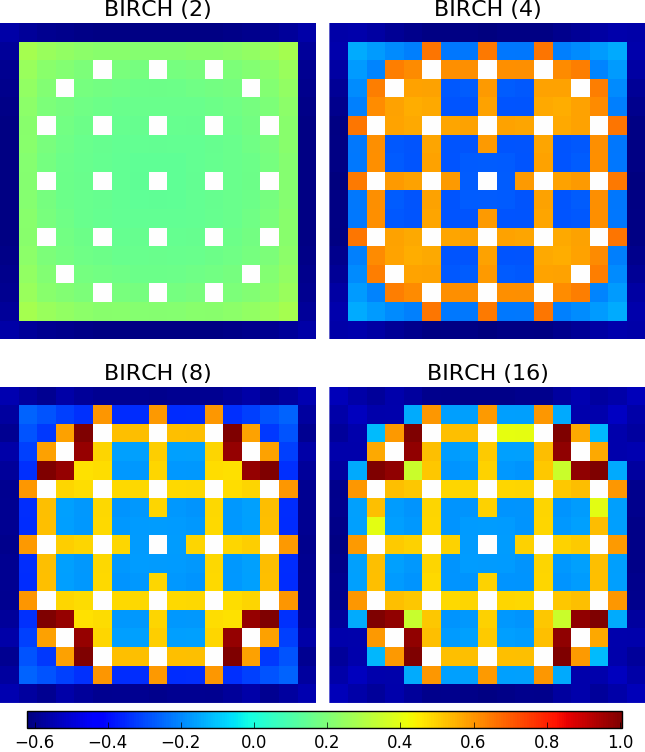
\includegraphics[width=0.9\linewidth]{figures/results/compare/assm-16/compare-capt}
\vspace{2mm}
\caption[U-238 capture rate comparison for a 1.6\% enriched assembly]{The percent relative deviation of U-238 capture rate spatial distributions for \textit{i}\ac{MGXS} and null homogenization for a 1.6\% enriched assembly.}
\label{fig:chap11-assm-1.6-capt-rates-comp}
\end{figure}

\clearpage

\begin{figure}[h!]
\centering
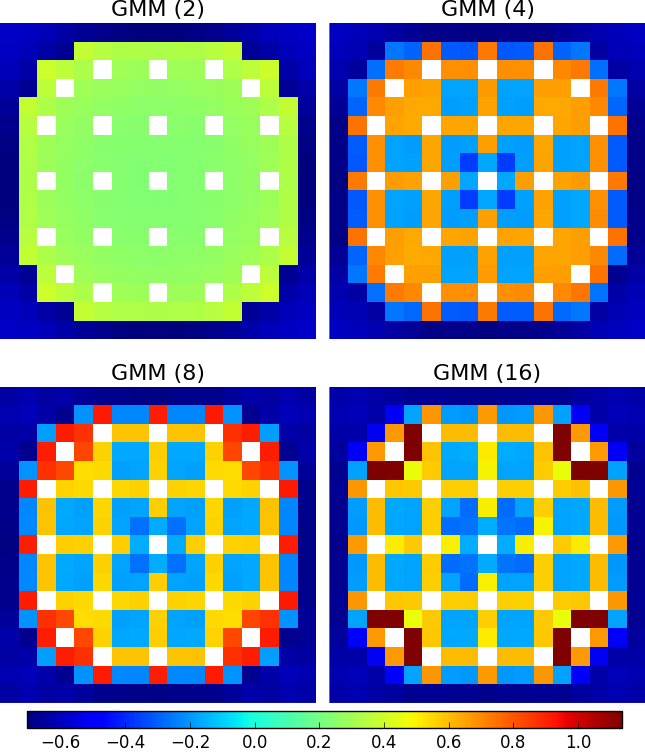
\includegraphics[width=0.9\linewidth]{figures/results/compare/assm-31/compare-capt}
\vspace{2mm}
\caption[U-238 capture rate comparison for a 3.1\% enriched assembly]{The percent relative deviation of U-238 capture rate spatial distributions for \textit{i}\ac{MGXS} and null homogenization for a 3.1\% enriched assembly.}
\label{fig:chap11-assm-3.1-capt-rates-comp}
\end{figure}

\clearpage

\begin{figure}[h!]
\centering
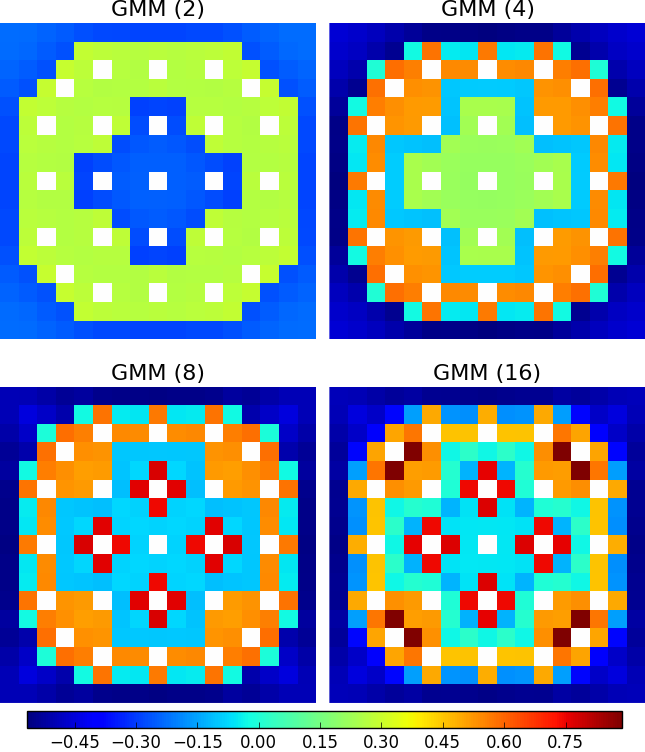
\includegraphics[width=0.9\linewidth]{figures/results/compare/assm-31-20BPs/compare-capt}
\vspace{2mm}
\caption[U-238 capture rate comparison for a 3.1\% enriched assembly with 20 BPs]{The percent relative deviation of U-238 capture rate spatial distributions for \textit{i}\ac{MGXS} and null homogenization for a 3.1\% enriched assembly with 20 \acp{BP}.}
\label{fig:chap11-assm-31-20BPs-capt-rates-comp}
\end{figure}
	
\clearpage

\begin{figure}[h!]
\centering
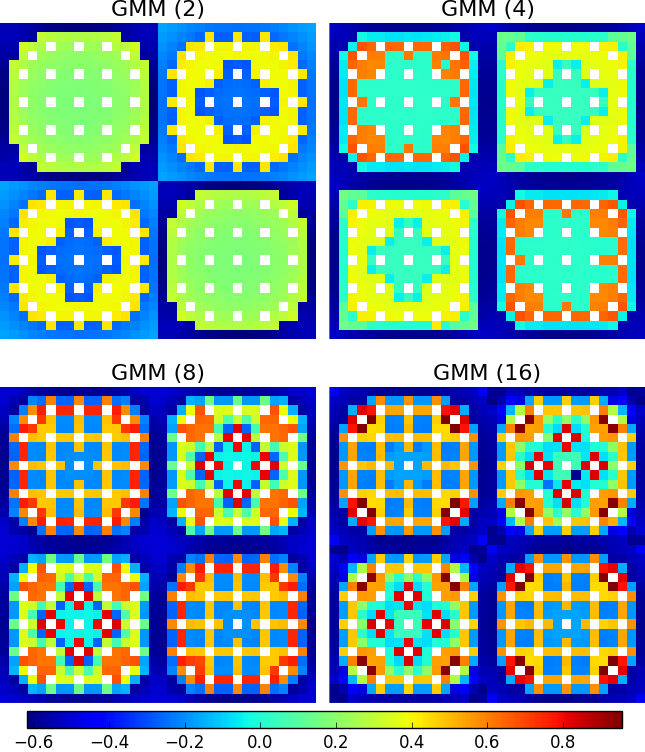
\includegraphics[width=0.9\linewidth]{figures/results/compare/2x2/compare-capt}
\vspace{2mm}
\caption[U-238 capture rate comparison for a 2$\times$2 colorset]{The percent relative deviation of U-238 capture rate spatial distributions for \textit{i}\ac{MGXS} and null homogenization for a 2$\times$2 colorset.}
\label{fig:chap11-2x2-capt-rates-comp}
\end{figure}

\clearpage

\begin{figure}[h!]
\centering
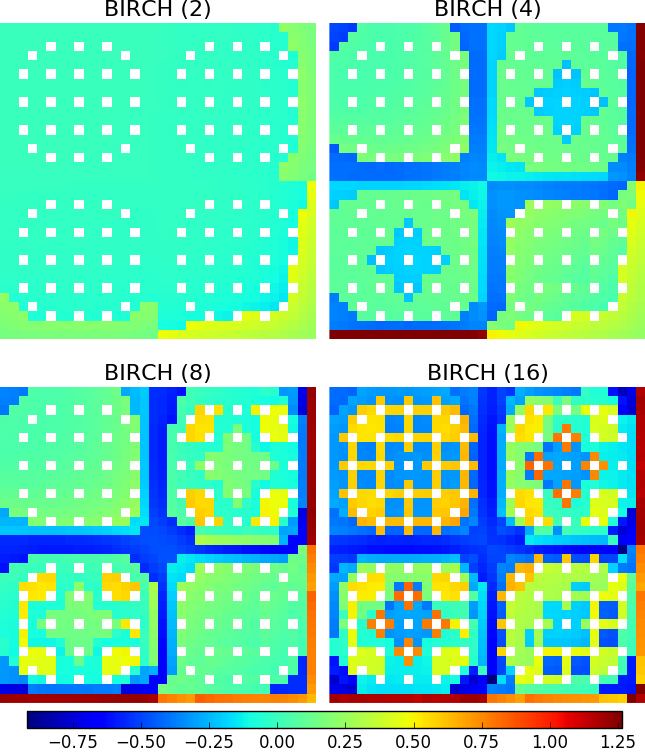
\includegraphics[width=0.9\linewidth]{figures/results/compare/reflector/compare-capt}
\vspace{2mm}
\caption[U-238 capture rate comparison for a 2$\times$2 colorset with reflector]{The percent relative deviation of U-238 capture rate spatial distributions for \textit{i}\ac{MGXS} and null homogenization for a 2$\times$2 colorset with a water reflector.}
\label{fig:chap11-refl-capt-rates-comp}
\end{figure}

\clearpage

\begin{figure}[h!]
\centering
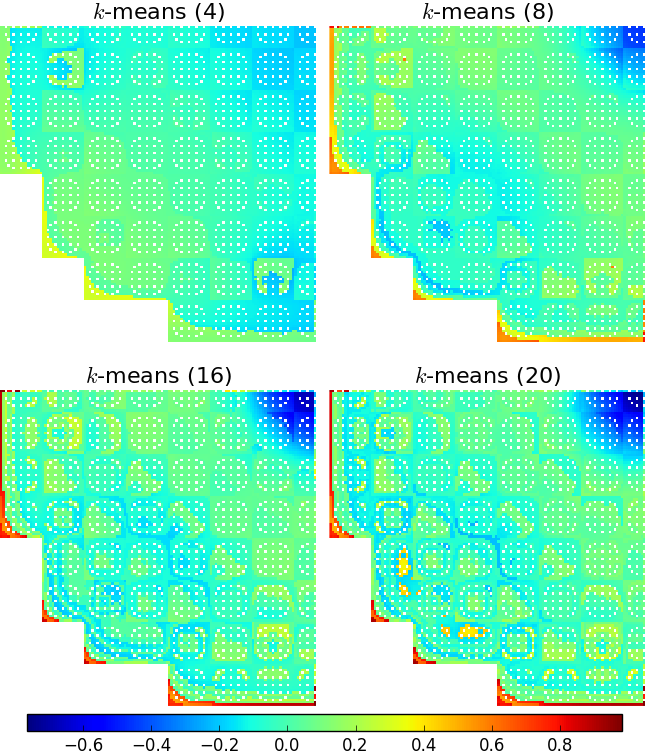
\includegraphics[width=0.9\linewidth]{figures/results/compare/full-core/compare-capt-kmeans}
\vspace{2mm}
\caption[U-238 capture rate comparison for the quarter core BEAVRS model]{The percent relative deviation of U-238 capture rate spatial distributions for \textit{i}\ac{MGXS} (\textit{with $k$-means}) and null homogenization for the quarter core BEAVRS model.}
\label{fig:chap11-full-core-capt-rates-kmeans-comp}
\end{figure}

\clearpage

\begin{figure}[h!]
\centering
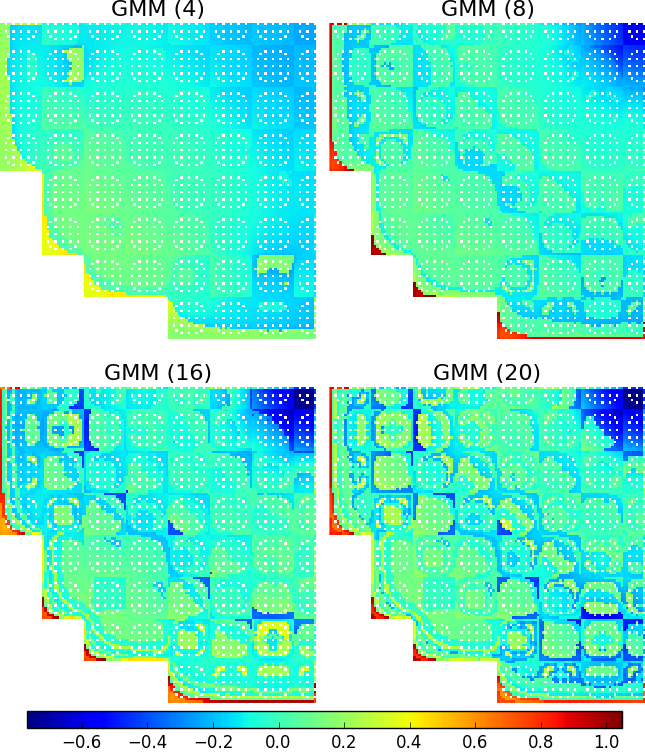
\includegraphics[width=0.9\linewidth]{figures/results/compare/full-core/compare-capt-gmm}
\vspace{2mm}
\caption[U-238 capture rate comparison for the quarter core BEAVRS model]{The percent relative deviation of U-238 capture rate spatial distributions for \textit{i}\ac{MGXS} (\textit{with \ac{GMM}}) and null homogenization for the quarter core BEAVRS model.}
\label{fig:chap11-full-core-capt-rates-gmm-comp}
\end{figure}

\clearpage

\begin{figure}[h!]
\centering
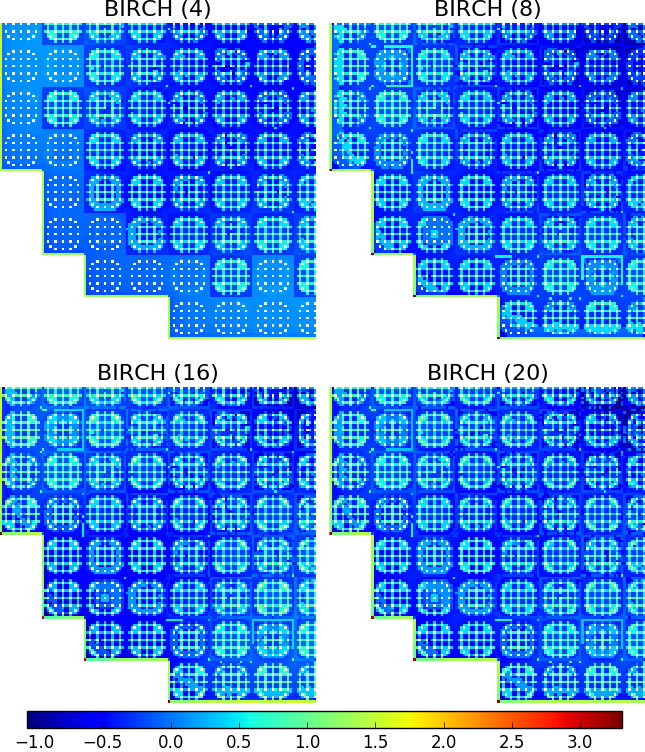
\includegraphics[width=0.9\linewidth]{figures/results/compare/full-core/compare-capt-birch}
\vspace{2mm}
\caption[U-238 capture rate comparison for the quarter core BEAVRS model]{The percent relative deviation of U-238 capture rate spatial distributions for \textit{i}\ac{MGXS} (\textit{with BIRCH}) and null homogenization for the quarter core BEAVRS model.}
\label{fig:chap11-full-core-capt-rates-birch-comp}
\end{figure}

\clearpage


%%%%%%%%%%%%%%%%%%%%%%%%%%%%%%%%%%%%%%%%%%%%%%%%%%%%%%%%%%%%%%%%%%%%%%%%%%%%%%%
\section{Convergence of OpenMOC Solutions}
\label{sec:chap11-converge}

This section attempts to determine the how quickly multi-group solutions converge with number of \ac{MC} particle histories simulated to generate \ac{MGXS}. In particular, this section quantifies the number of histories needed to sufficiently converge \ac{MGXS} for stable OpenMOC solutions with the null, degenerate and \textit{i}\ac{MGXS} spatial homogenization schemes for each of the six benchmarks. In addition, the convergence of the OpenMOC solutions are compared to the statistical uncertainties of the corresponding reference OpenMC calculation. This comparison is used to quantify how much faster a solution for a specified accuracy can be achieved with OpenMOC with \ac{MGXS} generated by OpenMC.

This section uses the \ac{MC} tally data generated by the same OpenMC simulations which generated \ac{MGXS} for Sec.~\ref{subsec:chap11-imgxs-results}. However, the \ac{MGXS} in this section are computed from \ac{MC} tally data stored as OpenMC \textit{statepoint} files for 100 different active batches. For the assembly and colorset benchmarks, 80\% of the statepoints were recorded at a logarithmically-spaced interval for the first 1 -- 1,000 active batches (10$^{5}$ -- 10$^{8}$ histories), while the remaining 20\% were recorded at a logarithmically-spaced interval for the final 1,000 -- 9,800 active batches (10$^{8}$ -- 10$^{9}$ histories). The OpenMC statepoints for the earliest batches contained \ac{MC} tally data with the largest statistical uncertainties, while the tallies for the latter batches had smaller statistical uncertainties. The different statepoints enabled a thorough evaluation of the sensitivity of OpenMOC's solutions to the statistical uncertainties of the \ac{MGXS}.

The clustering models were built using the most highly converged \ac{MC} tally data stored for the final active batch (\textit{i.e.}, the same data used to train the clustering models employed in Sec.~\ref{subsec:chap11-imgxs-results}). These clustering models were then \textit{re-applied} for spatial homogenization of the lesser converged \ac{MC} tally data from earlier active batches. This methodology permitted a \textit{best case} assessment of the OpenMOC accuracy one could hope to achieve if the ``best'' clustering model were accessible (\textit{i.e.}. the clustering model one would find from ``fully'' converged \ac{MC} tally data). It is important to note that this methodology is \textit{not} representative of how \textit{i}\ac{MGXS} would be deployed for \ac{MGXS} generation in a production setting. Nevertheless, it was a useful exercise to simply quantify the \textit{upper bound} on the acceleration achievable if an optimal \textit{i}\ac{MGXS} configuration were invented which could infer reliable cluster assignments from highly unconverged \ac{MC} tally data.

%The objective for \textit{i}\ac{MGXS} is to infer accurate \ac{MGXS} cluster assignments for each fuel pin instance from ``noisy'' \ac{MC} tally data to accelerate the simulation scheme.

The convergence rate of the eigenvalues generated with null, degenerate and \textit{i}\ac{MGXS} homogenization is presented in Sec.~\ref{subsec:chap11-eigenvalue-converge}. Likewise, the convergence of the U-238 capture rate relative errors is examined in Sec.~\ref{subsec:chap11-capture-converge} for each scheme.

%%%%%%%%%%%%%%%%%%%%%%%%%%%%%%%%%%%
\subsection{Eigenvalue Convergence}
\label{subsec:chap11-eigenvalue-converge}

The OpenMOC eigenvalues were compared to the reference OpenMC eigenvalues from Tab.~\ref{table:chap7-ref-eigenvalues} for each of the 100 active batches. The eigenvalue bias $\Delta\rho$ was computed from Eqn.~\ref{eqn:chap5-delta-rho} in units of \ac{pcm}. The batch-by-batch bias is presented in Figs.~\Crefrange{fig:chap11-assm-1.6-eigenvalue-converge}{fig:chap11-refl-eigenvalue-converge} for the individual assembly and 2$\times$2 colorset benchmarks. In particular, the bias is presented for null, degenerate and \textit{i}\ac{MGXS} homogenization with BIRCH clustering of 2, 4 and 10 clusters for the assemblies and periodic colorset, and for 2, 4 and 16 clusters for the colorset with a water reflector. The bias is highlighted for 10$^{5}$ -- 10$^{9}$ active histories for the assemblies and 10$^{6}$ -- 10$^{9}$ histories for the colorsets, respectively\footnote{A few hundred thousand histories were required to sufficiently converge the \ac{MGXS} for the colorsets to compute stable solutions with OpenMOC.}.

The biases converge to nearly the same value for all of the benchmarks and spatial homogenization schemes, as expected based on the converged eigenvalue biases tabulated in Sec.~\ref{subsec:chap11-imgxs-eigenvalues}. This is consistent with the fact that globally-integrated reaction rates are preserved for all schemes irregardless of the number of clusters modeled. Of particular note is that the bias for the null and \textit{i}\ac{MGXS} schemes are quite consistent even with as few as 10$^{5}$ particle histories. The bias for the degenerate scheme deviates by up 100 \ac{pcm}, but eventually converges to the null and \textit{i}\ac{MGXS} schemes with enough particle histories. The bias fluctuates on the order of 500 \ac{pcm} with fewer than 10$^{7}$ particle histories, but converges with 10$^{8}$ histories for all of the benchmarks and schemes.

A number of different factors may cause the eigenvalue to fluctuate and deviate between schemes for few particle histories. First, the statistical uncertainties of the \ac{MGXS} must be minimized in order to converge the OpenMOC eigenvaues. In addition, it should be recalled from Sec.~\ref{sec:chap3-mgxs-gen} that the \ac{MGXS} are generated from OpenMC using a mixture of track-length and analog tally estimators. In particular, the total, fission and capture \ac{MGXS} are computed with track-length estimators, while the scattering matrices and fission spectra are computed from analog estimators since they depend on the neutron's outgoing energy at each interaction. Although both track-length and analog estimators will converge to the same expected value, analog estimators will converge more slowly. As a result, neutron balance will not be preserved for \ac{MGXS} computed from a mixture of track-length and analog estimators without a sufficient number of simulated histories. This issue was the a key motivating factor for Nelson's Nuclear Data PreProcessor (NDPP)~\cite{nelson2014improved} to enable track-length estimators for multi-group scattering matrices and fission spectra. Methods  such as NDPP may be a fruitful area of future research to enable faster converging eigenvalues from \ac{MGXS} generated with \ac{MC}.

\begin{emphbox}
\textbf{The null, degenerate and \textit{i}\ac{MGXS} schemes converge to the same eigenvalue bias with 10$^{8}$ particle histories for the assembly and colorset benchmarks.}
\end{emphbox}

%-why do the plots start at 10^5 for the assemblies, and 10^6 for the colorsets???
%  -because 100,000 particles led to NaNs for the reflector and colorset benchmarks

\begin{figure}[h!]
\centering
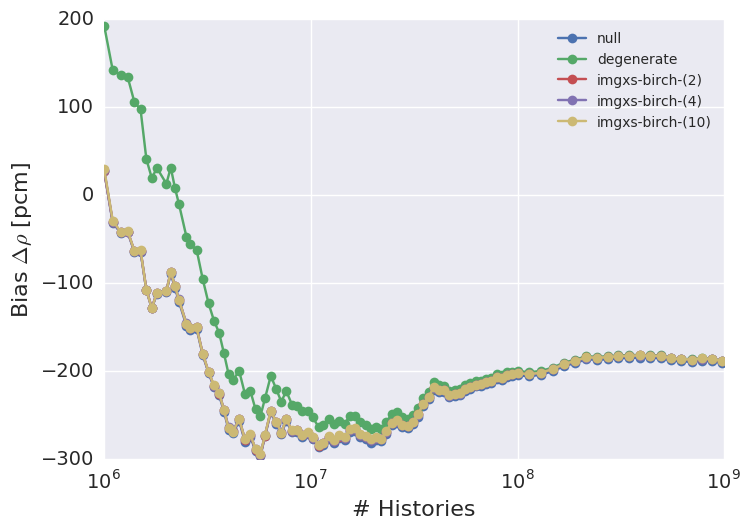
\includegraphics[width=0.88\linewidth]{figures/results/convergence/assm-16/keff-bias-evo}
\vspace{2mm}
\caption[Eigenvalue bias covergence for a 1.6\% enriched assembly]{Convergence of the eigenvalue bias for the 1.6\% enriched assembly.}
\label{fig:chap11-assm-1.6-eigenvalue-converge}
\end{figure}

\begin{figure}[h!]
\centering
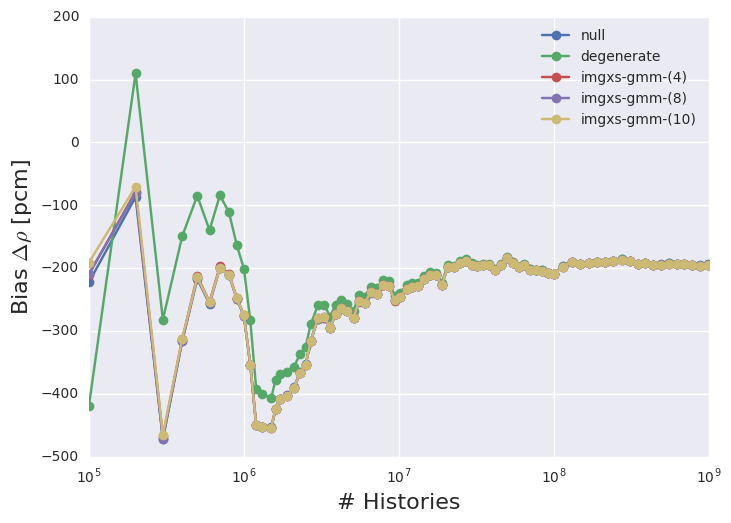
\includegraphics[width=0.88\linewidth]{figures/results/convergence/assm-31/keff-bias-evo}
\vspace{2mm}
\caption[Eigenvalue bias covergence for a 3.1\% enriched assembly]{Convergence of the eigenvalue bias for the 3.1\% enriched assembly.}
\label{fig:chap11-assm-3.1-eigenvalue-converge}
\end{figure}

\begin{figure}[h!]
\centering
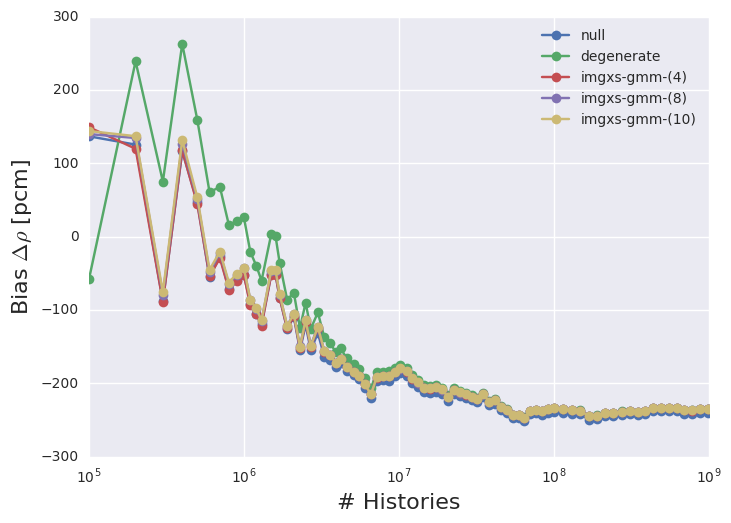
\includegraphics[width=0.88\linewidth]{figures/results/convergence/assm-31-20BPs/keff-bias-evo}
\vspace{2mm}
\caption[Eigenvalue bias covergence for a 3.1\% enriched assembly with 20 \acp{BP}]{Convergence of the eigenvalue bias for the 3.1\% enriched assembly with 20 \acp{BP}.}
\label{fig:chap11-assm-3.1-20BPs-eigenvalue-converge}
\end{figure}

\begin{figure}[h!]
\centering
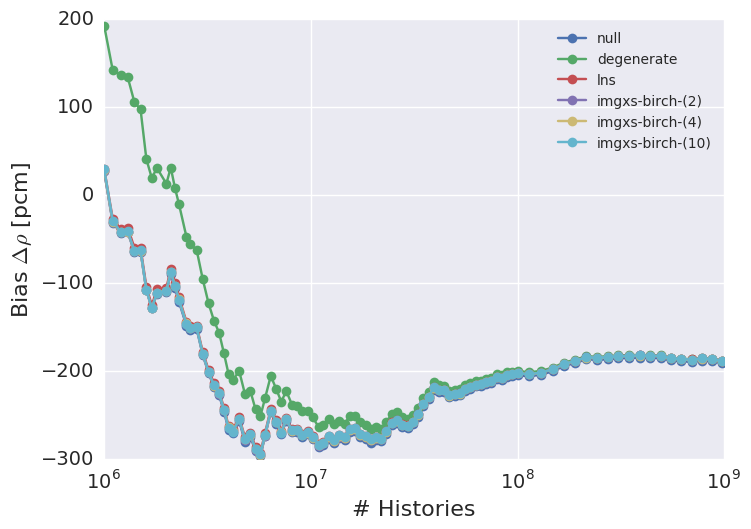
\includegraphics[width=0.88\linewidth]{figures/results/convergence/2x2/keff-bias-evo}
\vspace{2mm}
\caption[Eigenvalue bias covergence for a 2$\times$2 colorset]{Convergence of the eigenvalue bias for the periodic colorset.}
\label{fig:chap11-2x2-eigenvalue-converge}
\end{figure}

\begin{figure}[h!]
\centering
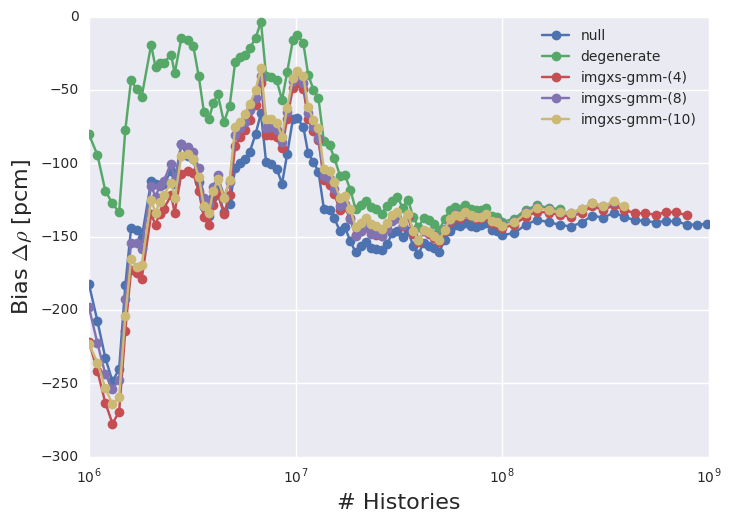
\includegraphics[width=0.88\linewidth]{figures/results/convergence/reflector/keff-bias-evo}
\vspace{2mm}
\caption[Eigenvalue bias covergence for a 2$\times$2 colorset with reflector]{Convergence of the eigenvalue bias for the colorset with a water reflector.}
\label{fig:chap11-refl-eigenvalue-converge}
\end{figure}

\clearpage

%%%%%%%%%%%%%%%%%%%%%%%%%%%%%%%%%%%%%%%%%%%
\subsection{U-238 Capture Rate Convergence}
\label{subsec:chap11-capture-converge}

first paragraph: outline
-Figs.~\Crefrange{fig:chap11-assm-1.6-capture-converge}{fig:chap11-refl-capture-converge}
  -individual assemblies and colorsets
-use BIRCH clustering with 2, 4 and 10 clusters for assemblies and periodic colorset
-use BIRCH clustering with 2, 4 and 16 clusters for reflected colorset
-openmc 1-sigma uncertainty is reported relative to the mean
  -not a direct comparison to the percentage relative error reported for OpenMOC

second paragraph: analysis
-smoother convergence for mean than for the max error
-openmc will converge to zero
-null, degenerate and \textit{i}\ac{MGXS} schemes will not converge to some non-zero bias
  -accounts for various approx (energy, spatial and angular discretization)
-convergence of null
  -null is stable with 100,000 particles for assemblies and 1,000,000 particle for colorsets
-convergence of degenerate
  -takes over 100,000,000 particles to converge for assemblies
  -takes at least 1,000,000,000 particles to converge for colorsets (not even shown on plots)
-convergence of \textit{i}\ac{MGXS}
  -the more clusters, the longer it takes to converge
  -the more clusters, the lower the final converged value (smaller bias)
  -the more clusters, the more erratic the convergence
    -would be interesting to look at alternatives to track density-weighting
    -how about taking the median MGXS from each cluster?
      -would be less sensitive to outliers and potentially more ``robust''
      -but wouldn't preserve global reactivity
    -recall argument about LNS - uneven number of fuel pin instances assigned to each cluster
      -clusters with the fewest pins will be most constraining on convergence
-convergence of openmc to degenerate
  -openmc max always less than degenerate
  -but openmc mean greater than degenerate for few particles
    -eventually drops below as degenerate converges to non-zero bias
  -takes perhaps 30,000,000 particles for max to reach degenerate for assemblies (60,000,000 for colorsets?)
  -but over 500,000,000 particles for mean to reach degenerate

\begin{figure}[h!]
\centering
\begin{subfigure}{\textwidth}
  \centering
  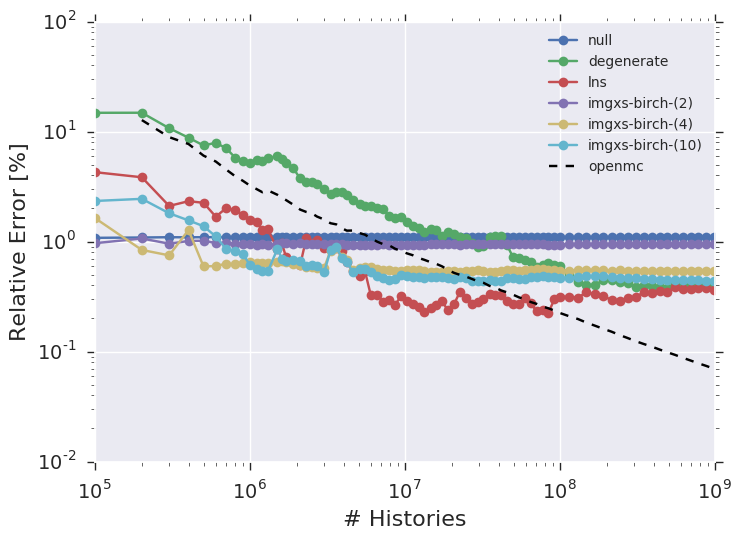
\includegraphics[width=0.9\linewidth]{figures/results/convergence/assm-16/max-capt-err-evo}
  \caption{}
  \label{fig:chap11-assm-1.6-capture-converge-max}
\end{subfigure}
\begin{subfigure}{\textwidth}
  \centering
  \includegraphics[width=0.9\linewidth]{figures/results/convergence/assm-16/mean-capt-err-evo}
  \caption{}
  \label{fig:chap11-assm-1.6-capture-converge-mean}
\end{subfigure}
\vspace{2mm}
\caption[Fission rate covergence for a 1.6\% enriched assembly]{Convergence of the max (a) and mean (b) absolute U-238 capture rate percent relative errors for a 1.6\% enriched assembly.}
\label{fig:chap11-assm-1.6-capture-converge}
\end{figure}

\begin{figure}[h!]
\centering
\begin{subfigure}{\textwidth}
  \centering
  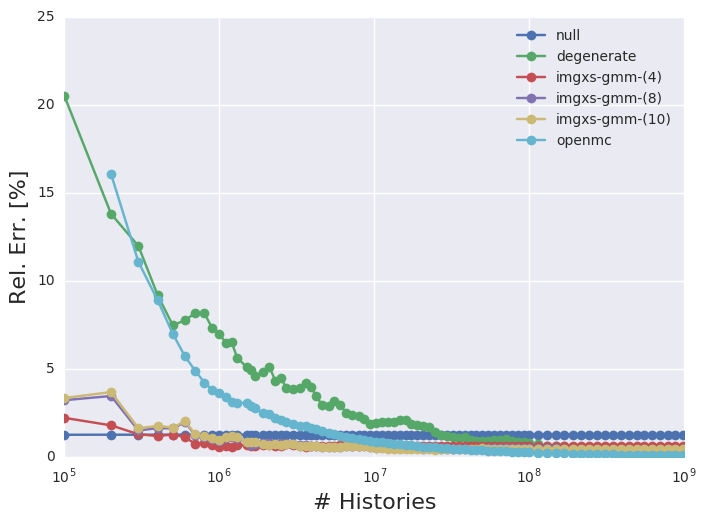
\includegraphics[width=0.9\linewidth]{figures/results/convergence/assm-31/max-capt-err-evo}
  \caption{}
  \label{fig:chap11-assm-3.1-capture-converge-max}
\end{subfigure}
\begin{subfigure}{\textwidth}
  \centering
  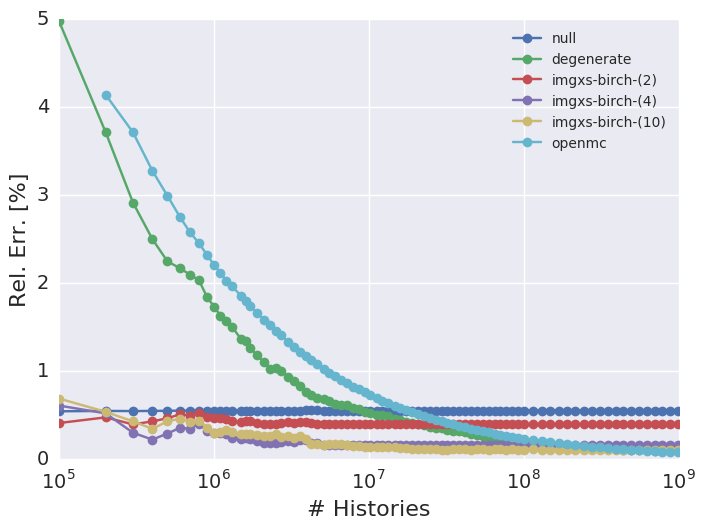
\includegraphics[width=0.9\linewidth]{figures/results/convergence/assm-31/mean-capt-err-evo}
  \caption{}
  \label{fig:chap11-assm-3.1-capture-converge-mean}
\end{subfigure}
\vspace{2mm}
\caption[Fission rate covergence for a 3.1\% enriched assembly]{Convergence of the max (a) and mean (b) absolute U-238 capture rate percent relative errors for a 3.1\% enriched assembly.}
\label{fig:chap11-assm-3.1-capture-converge}
\end{figure}

\begin{figure}[h!]
\centering
\begin{subfigure}{\textwidth}
  \centering
  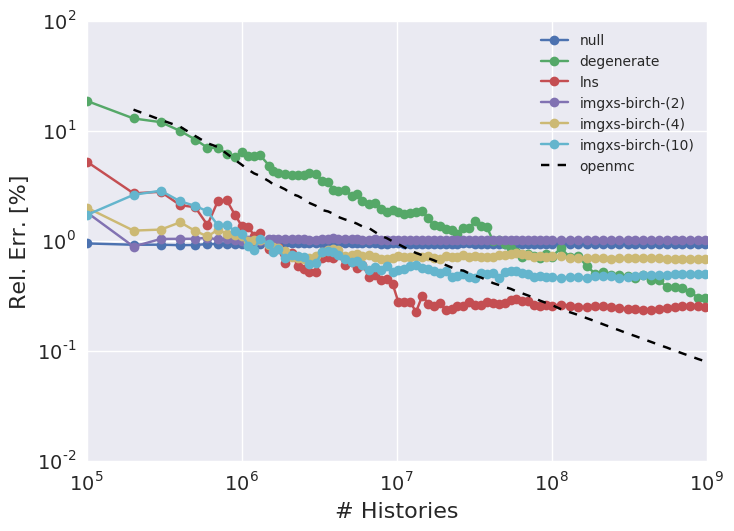
\includegraphics[width=0.9\linewidth]{figures/results/convergence/assm-31-20BPs/max-capt-err-evo}
  \caption{}
  \label{fig:chap11-assm-3.1-20BPs-capture-converge-max}
\end{subfigure}
\begin{subfigure}{\textwidth}
  \centering
  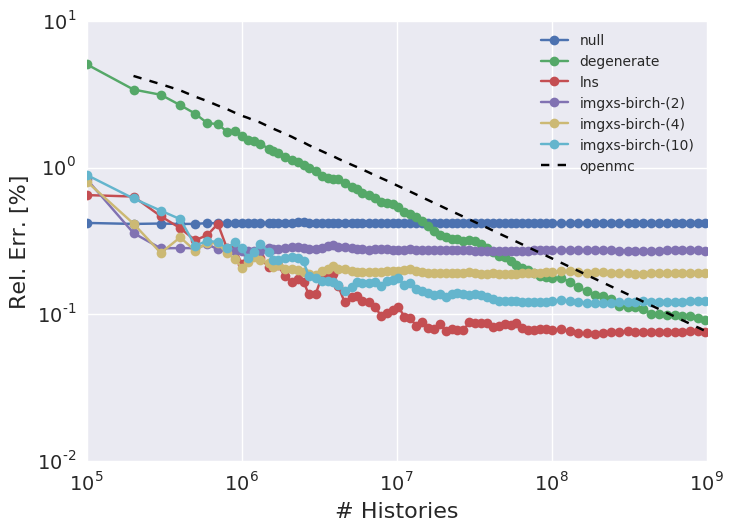
\includegraphics[width=0.9\linewidth]{figures/results/convergence/assm-31-20BPs/mean-capt-err-evo}
  \caption{}
  \label{fig:chap11-assm-3.1-20BPs-capture-converge-mean}
\end{subfigure}
\vspace{2mm}
\caption[Fission rate covergence for a 3.1\% enriched assembly with 20 \acp{BP}]{Convergence of the max (a) and mean (b) absolute U-238 capture rate percent relative errors for a 3.1\% enriched assembly with 20 \acp{BP}.}
\label{fig:chap11-assm-3.1-20BPs-capture-converge}
\end{figure}

\begin{figure}[h!]
\centering
\begin{subfigure}{\textwidth}
  \centering
  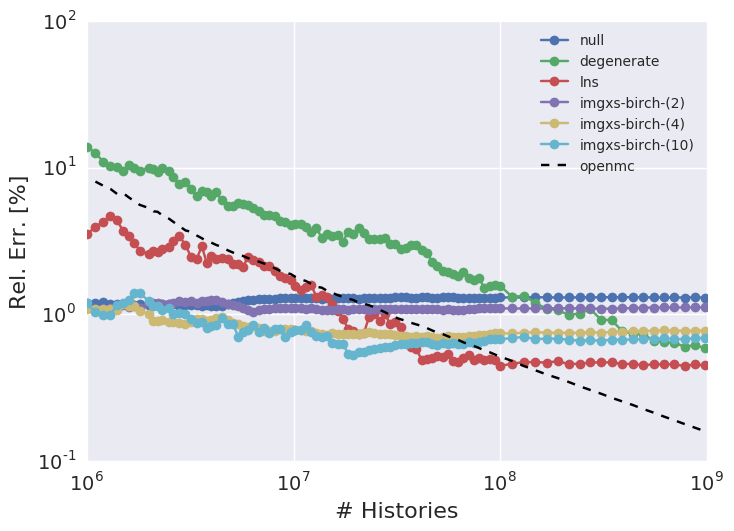
\includegraphics[width=0.9\linewidth]{figures/results/convergence/2x2/max-capt-err-evo}
  \caption{}
  \label{fig:chap11-2x2-capture-converge-max}
\end{subfigure}
\begin{subfigure}{\textwidth}
  \centering
  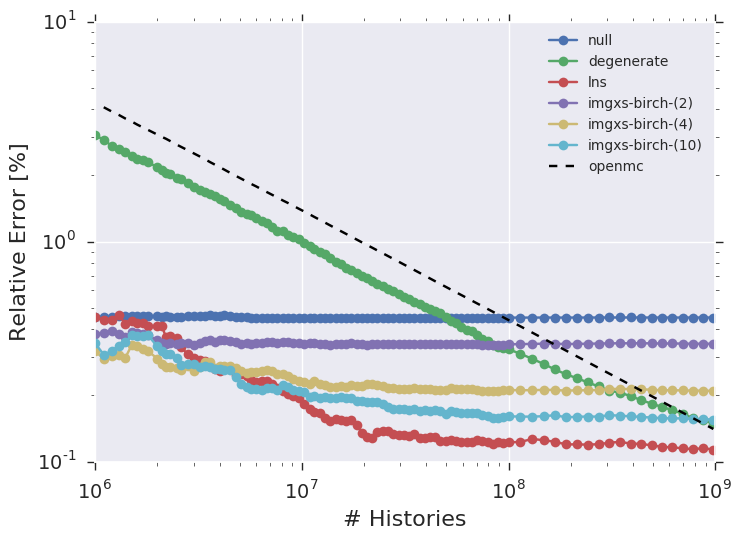
\includegraphics[width=0.9\linewidth]{figures/results/convergence/2x2/mean-capt-err-evo}
  \caption{}
  \label{fig:chap11-2x2-capture-converge-mean}
\end{subfigure}
\vspace{2mm}
\caption[Fission rate covergence for a 2$\times$2 colorset]{Convergence of the max (a) and mean (b) absolute U-238 capture rate percent relative errors for a 2$\times$2 colorset.}
\label{fig:chap11-2x2-capture-converge}
\end{figure}

\begin{figure}[h!]
\centering
\begin{subfigure}{\textwidth}
  \centering
  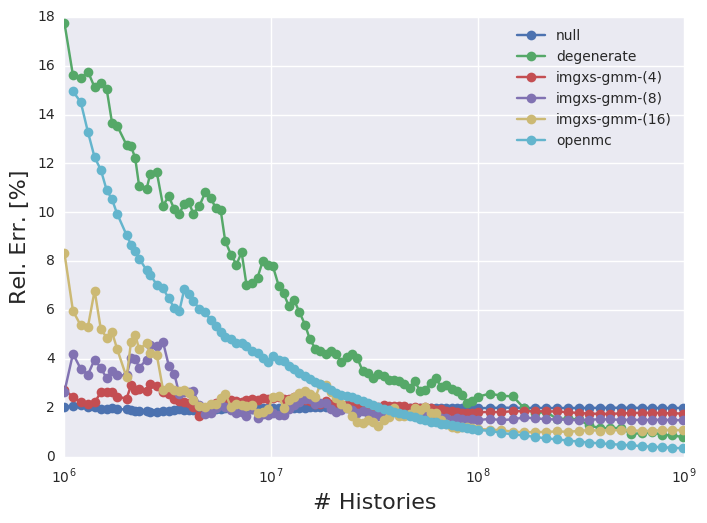
\includegraphics[width=0.9\linewidth]{figures/results/convergence/reflector/max-capt-err-evo}
  \caption{}
  \label{fig:chap11-refl-capture-converge-max}
\end{subfigure}
\begin{subfigure}{\textwidth}
  \centering
  \includegraphics[width=0.9\linewidth]{figures/results/convergence/reflector/mean-capt-err-evo}
  \caption{}
  \label{fig:chap11-refl-capture-converge-mean}
\end{subfigure}
\vspace{2mm}
\caption[Fission rate covergence for a 2$\times$2 colorset with reflector]{Convergence of the max (a) and mean (b) absolute U-238 capture rate percent relative errors for a 2$\times$2 colorset with a water reflector.}
\label{fig:chap11-refl-capture-converge}
\end{figure}

-full core plots

SUMMARY BOX


%%%%%%%%%%%%%%%%%%%%%%%%%%%%%%%%%%%%%%%%%%%%%%%%%%%%%%%%%%%%%%%%%%%%%%%%%%%%%%%
\section{Evaluation of Model Selection Techniques}
\label{sec:chap11-model-select}

first paragraph: objective
-recall Sec.~\ref{sec:chap10-model-select}
-model selection needed to select number of clusters
  -can only evaluate clustering models with respect to the \ac{MC} tally data
  -don't have access to either:
    1) the ``true'' cluster labels
    2) the OpenMOC-OpenMC error
-can use intra-cluster and inter-cluster similarities
-can use likelihood and regularization (BIC) to balance bias-variance tradeoff

second paragraph: outline
-evaluate each heuristic with the 1.6\% enr assm and 2$\times$2 colorset with water reflector
-Sec.~\ref{subsec:chap11-db-index} Davies-Bouldin indices
-Sec.~\ref{subsec:chap11-dunn-index} Dunn indices
-Sec.~\ref{subsec:chap11-ch-index} Calinski-Harabaz indices
-Sec.~\ref{subsec:chap11-silhouette-coeff} silhouette coefficients
-Sec.~\ref{subsec:chap11-bic} Bayesian Information Criterion

-consider that cross-validation could make these heuristics more robust and less erratic
  -recall Sec.~\ref{subsec:chap10-cross-validate}
-could compare cluster labels to those from LNS (use LNS as the ``ground truth'')
-make axes labels clearer

%%%%%%%%%%%%%%%%%%%%%%%%%%%%%%%%%
\subsection{Davies-Bouldin Index}
\label{subsec:chap11-db-index}

first paragraph: outline and analysis
-recall Sec.~\ref{subsec:chap10-db-index}
-Figs.~\Crefrange{fig:chap11-assm-16-db-index}{fig:chap11-refl-db-index}
-want to minimize DB index
-minima are all for a single cluster
-can use ``elbow'' method to look at point at which DB index shoots up
  -around 10 clusters for assm
  -around 9 clusters for colorset
-not clear how one would use these results to create a robust, automated model selection system
  -perhaps CV would help??

\begin{figure}[h!]
\centering
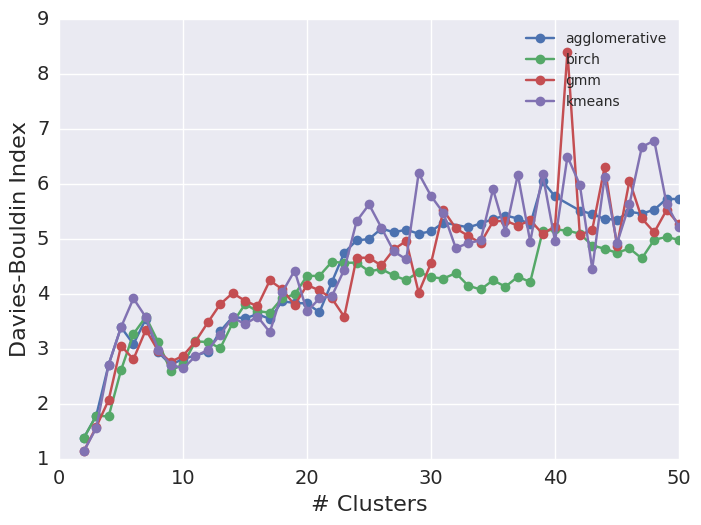
\includegraphics[width=0.87\linewidth]{figures/results/model-select/assm-16/db-combined-U238-capture-1}
\vspace{2mm}
\caption[Davies-Bouldin indices for the 1.6\% enriched assembly]{Davies-Bouldin indices for the 1.6\% enriched assembly.}
\label{fig:chap11-assm-16-db-index}
\end{figure}

\begin{figure}[h!]
\centering
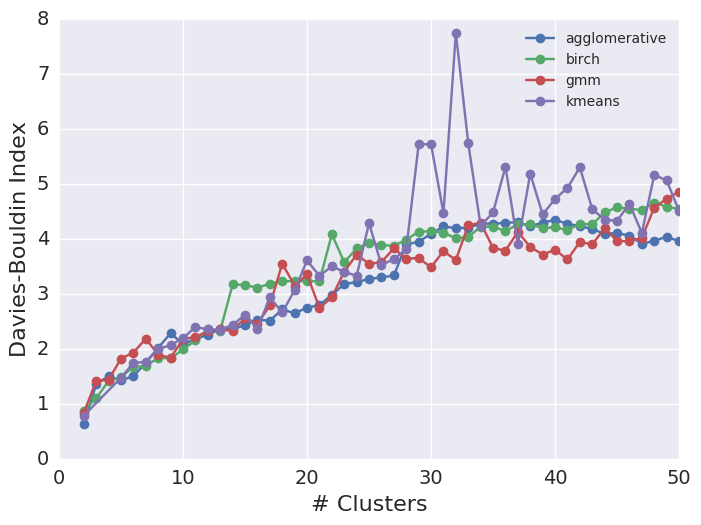
\includegraphics[width=0.87\linewidth]{figures/results/model-select/reflector/db-combined-U238-nu-fission-1}
\vspace{2mm}
\caption[Davies-Bouldin indices for the 2$\times$2 colorset with reflector]{Davies-Bouldin indices for the 2$\times$2 colorset with a water reflector.}
\label{fig:chap11-refl-db-index}
\end{figure}

%%%%%%%%%%%%%%%%%%%%%%%
\subsection{Dunn Index}
\label{subsec:chap11-dunn-index}

first paragraph: outline and analysis
-recall Sec.~\ref{subsec:chap10-dunn-index}
-Figs.~\Crefrange{fig:chap11-assm-16-dunn-index}{fig:chap11-refl-dunn-index}
-want to maximize Dunn index
-Dunn index is constrained by the most poorly behaving cluster
  -leads to the step-like behavior
    -indicates that the most poorly behaving cluster is not always refined with each successive cluster added to the models
-again not clear how one would use these results to create a robust, automated model selection system
  -perhaps CV would help??

\begin{figure}[h!]
\centering
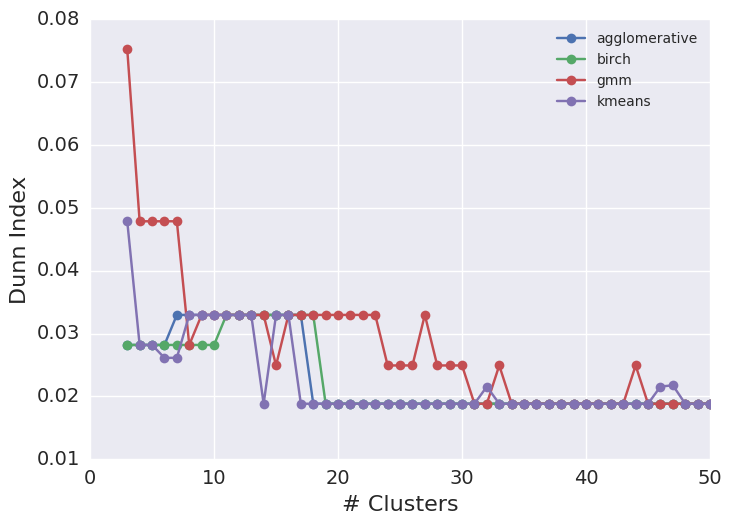
\includegraphics[width=0.87\linewidth]{figures/results/model-select/assm-16/dunn-combined-U238-capture-1}
\vspace{2mm}
\caption[Dunn indices for the 1.6\% enriched assembly]{Dunn indices for the 1.6\% enriched assembly.}
\label{fig:chap11-assm-16-dunn-index}
\end{figure}

\begin{figure}[h!]
\centering
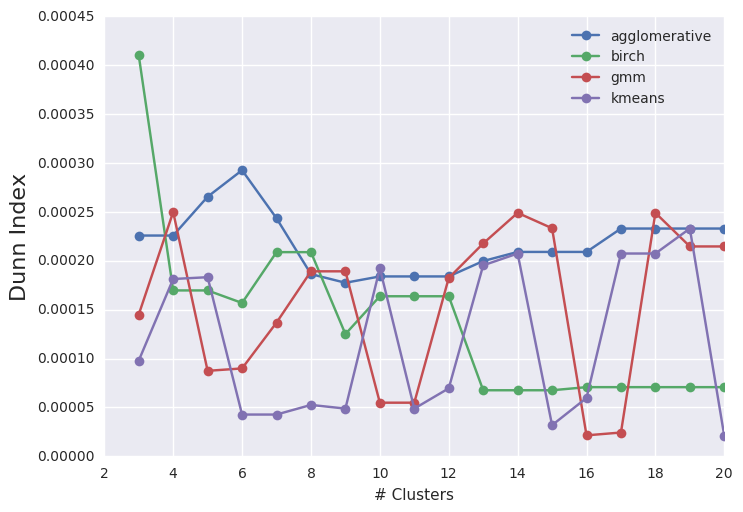
\includegraphics[width=0.87\linewidth]{figures/results/model-select/reflector/dunn-combined-U238-nu-fission-1}
\vspace{2mm}
\caption[Dunn indices for the 2$\times$2 colorset with reflector]{Dunn indices for the 2$\times$2 colorset with a water reflector.}
\label{fig:chap11-refl-dunn-index}
\end{figure}

%%%%%%%%%%%%%%%%%%%%%%%%%%%%%%%%%%%
\subsection{Calinski-Harabaz Index}
\label{subsec:chap11-ch-index}

first paragraph: outline and analysis
-recall Sec.~\ref{subsec:chap10-calinski-harabaz}
-Figs.~\Crefrange{fig:chap11-assm-16-ch-index}{fig:chap11-refl-ch-index}
-want to maximize CH index
-more smoothly varying behavior
-more tightly bunched behavior for the four algorithms than was the case for Dunn and DB
-index doesn't seem to peak at 20 clusters for CH index
-seems to reach plateau after 10 -- 14 clusters for colorset
-again not clear how one would use these results to create a robust, automated model selection system
  -perhaps CV would help??

\begin{figure}[h!]
\centering
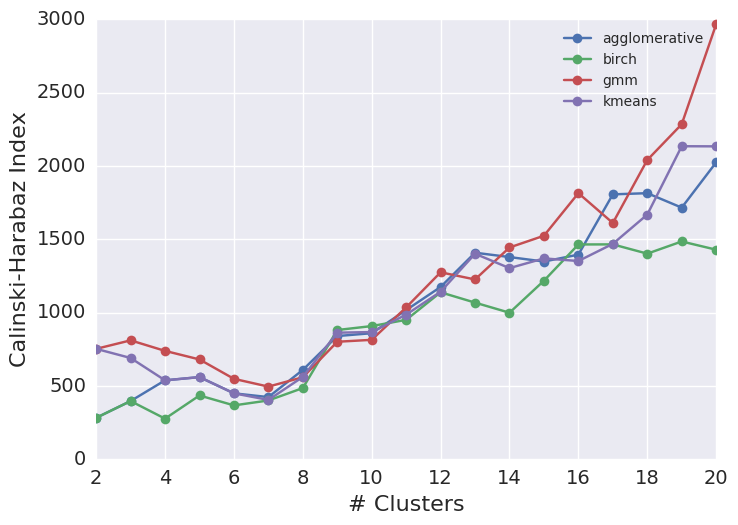
\includegraphics[width=0.87\linewidth]{figures/results/model-select/assm-16/ch-combined-U238-capture-1}
\vspace{2mm}
\caption[Calinski-Harabaz indices for the 1.6\% enriched assembly]{Calinski-Harabaz indices for the 1.6\% enriched assembly.}
\label{fig:chap11-assm-16-ch-index}
\end{figure}

\begin{figure}[h!]
\centering
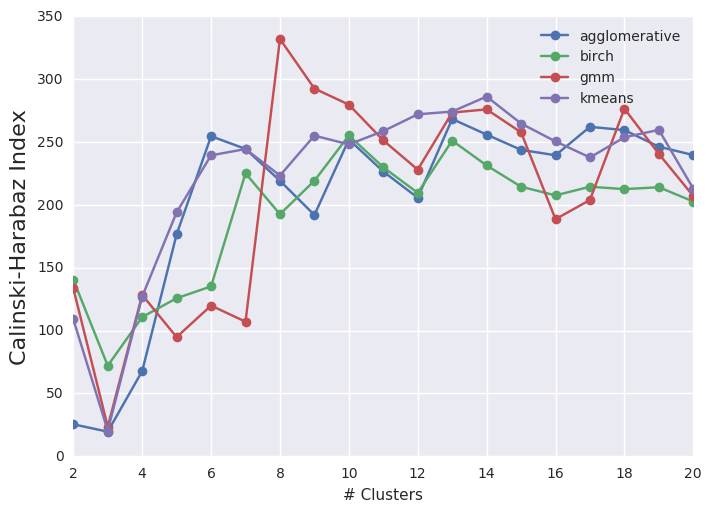
\includegraphics[width=0.87\linewidth]{figures/results/model-select/reflector/ch-combined-U238-nu-fission-1}
\vspace{2mm}
\caption[Calinski-Harabaz indices for the 2$\times$2 colorset with reflector]{Calinski-Harabaz indices for the 2$\times$2 colorset with a water reflector.}
\label{fig:chap11-refl-ch-index}
\end{figure}

%%%%%%%%%%%%%%%%%%%%%%%%%%%%%%%%%%%
\subsection{Silhouette Coefficient}
\label{subsec:chap11-silhouette-coeff}

first paragraph: outline and analysis
-recall Sec.~\ref{subsec:chap10-silhouette-coeff}
-Figs.~\Crefrange{fig:chap11-assm-16-silhouette-coeff}{fig:chap11-refl-silhouette-coeff}
-want to maximize silhouette coeff
-coeffs peak for a single cluster for both assm and colorset
-more tightly bunched behavior for the four algorithms than was the case for Dunn and DB, but less so than for CH
-again not clear how one would use these results to create a robust, automated model selection system
  -perhaps CV would help??

\begin{figure}[h!]
\centering
\includegraphics[width=0.87\linewidth]{figures/results/model-select/assm-16/silhouette-combined-U238-capture-1}
\vspace{2mm}
\caption[Silhouette coefficients for the 1.6\% enriched assembly]{Silhouette coefficients for the 1.6\% enriched assembly.}
\label{fig:chap11-assm-16-silhouette-coeff}
\end{figure}

\begin{figure}[h!]
\centering
\includegraphics[width=0.87\linewidth]{figures/results/model-select/reflector/silhouette-combined-U238-nu-fission-1}
\vspace{2mm}
\caption[Silhouette coefficients for the 2$\times$2 colorset with reflector]{Silhouette coefficients for the 2$\times$2 colorset with a water reflector.}
\label{fig:chap11-refl-silhouette-coeff}
\end{figure}

%%%%%%%%%%%%%%%%%%%%%%%%%%%%%%%%%%%%%%%%%%%
\subsection{Bayesian Information Criterion}
\label{subsec:chap11-bic}

first paragraph: outline and analysis
-recall Sec.~\ref{subsec:chap10-bic}
-Figs.~\Crefrange{fig:chap11-assm-16-bic}{fig:chap11-refl-bic}
-want to minimize BIC
-BIC only has closed form solution for \ac{GMM}
-BIC is much more smoothly varying with the number of clusters than the preceding metrics
-BIC doesn't seem to reach a minima even with 20 clusters
  -though seems to be leveling for the single assm
  -would eventually start to increase due to growth of second penalty term in the BIC expression
-can see the impact of diminishing returns in the BIC
  -the first 5 clusters causes the BIC to decrease the most
-could foresee a method which would choose the number of clusters using this method
  -might choose based on the fractional change in the BIC with each successive cluster

\begin{figure}[h!]
\centering
\includegraphics[width=0.87\linewidth]{figures/results/model-select/assm-16/bic-combined-U238-capture-1}
\vspace{2mm}
\caption[Silhouette coefficients for the 1.6\% enriched assembly]{Bayesian Information Criteria (BIC) for the 1.6\% enriched assembly.}
\label{fig:chap11-assm-16-bic}
\end{figure}

\begin{figure}[h!]
\centering
\includegraphics[width=0.87\linewidth]{figures/results/model-select/reflector/bic-combined-U238-nu-fission-1}
\vspace{2mm}
\caption[BIC for the 2$\times$2 colorset with reflector]{Bayesian Information Criteria (BIC) for the 2$\times$2 colorset with a water reflector.}
\label{fig:chap11-refl-bic}
\end{figure}

SUMMARY BOX!!!

%%%%%%%%%%%%%%%%%%%%%%%%%%%%%%%%%%%%%%%%%%%%%%%%%%%%%%%%%%%%%%%%%%%%%%%%%%%%%%%
\section{Synthesis}
\label{sec:chap11-synthesis}

first paragraph:
-bring it all together - what does it all mean??
  -refer to Fig.~\ref{fig:chap10-flow-chart}
  -recall dual goals - runtime, MC accuracy, etc.
-quantify how much faster \textit{i}\ac{MGXS} would be then full core MC
  -Tab.~\ref{table:chap11-runtimes}
-OpenMOC runtimes for litmus-only feature selection with ? with ? clusters

second paragraph:
-refer to Kord's suggestions about comparing to case where each individual sub-component is modeled
 -each unique assm
 -each colorset
 -corner-baffle case

-define a Figure of merit per Kord's suggestion
-add rel. err. and uncertainty to the table

%OpenMC particles / sec / core
%benchmark         no MGXs        MGXS
%1.6               2673.3         1154.4
%3.1               3012.9         1265.1
%3.1 BPs           3051.4         1011.4
%2x2               2976.3          784.9
%reflector         3004.6          795.6
%quarter core      2361.5          622.2

-use particle tracking rate to compute total time
  -read number of batches from the convergence plots as the max(max err,mean err) <= degenerate err
  -multiply number of batches by particle tracking rate
  -this uses the tracking rate without MGXS for the ``reference''
  -this use the tracking rate with MGXS for all others
  -10 clusters each???

\begin{table}[ht!]
  \centering
  \caption[Computational resource requirements for each simulation approach]{The computational resources needed for various simulation approaches to reach the level of accuracy achieved with degenerate spatial homogenization.}
  \small
  \label{table:chap11-runtimes}
  \vspace{6pt}
  \begin{tabular}{l l R{2.5cm} R{1.5cm} S[table-format=3.2] S[table-format=3.2] S[table-format=3.2]}
  \toprule
  \rowcolor{lightgray}
  & & & \multicolumn{3}{c}{\cellcolor{lightgray} \bf Runtime [core-hours]} \\
  \multirow{-2}{*}{\cellcolor{lightgray} \bf Benchmark} &
  \multirow{-2}{*}{\cellcolor{lightgray} \bf Scheme} &
  \multirow{-2}{*}{\cellcolor{lightgray} \bf \# Particles} &
  \multirow{-2}{*}{\cellcolor{lightgray} \bf Rel. Err. [\%]} &
  \multicolumn{1}{c}{\cellcolor{lightgray} \bf OpenMC} &
  \multicolumn{1}{c}{\cellcolor{lightgray} \bf OpenMOC} &
  \multicolumn{1}{c}{\cellcolor{lightgray} \bf Total} \\
  \midrule
\multirow{4}{*}{\parbox{2.5cm}{1.6\% Assm}} & Reference & 550,000,000 & & 57.2 & & 57.2 \\
& Null & 100,000 & &  0.02 & 0.36 & 0.38 \\
& Degenerate & 115,000,000 & & 27.7 & 0.40 & 28.1 \\
& \textit{i}\ac{MGXS} & 4,000,000 & & 0.96 & 0.38 & 1.34 \\
  \midrule
\multirow{4}{*}{\parbox{2.5cm}{3.1\% Assm}} & Reference & 550,000,000 & & 50.7 & & 50.7 \\
& Null & 100,000 & & 0.02 & 0.40 & 0.42 \\
& Degenerate & 115,000,000 & & 25.3 & 0.40 & 25.7 \\
& \textit{i}\ac{MGXS} & 4,000,000 & & 0.88 & 0.37 & 1.25 \\
  \midrule
\multirow{4}{*}{\parbox{2.5cm}{3.1\% Assm w/ 20 \acp{BP}}} & Reference & 550,000,000 & & 50.1 & & 50.1 \\
& Null & 100,000 & & 0.02 & 0.41 & 0.43 \\
& Degenerate & 115,000,000 & & 27.7 & 0.41 & 28.1 \\
& \textit{i}\ac{MGXS} & 4,000,000 & & 0.96 & 0.42 & 1.38 \\
  \midrule
\multirow{4}{*}{\parbox{2.5cm}{2$\times$2 Colorset}} & Reference & 8,755,000 & & 81.7 & & 81.7 \\
& Null & 100,000 & & 0.04 & 2.00 & 2.03 \\
& Degenerate & 700,000,000 & & 248 & 2.29 & 250 \\
& \textit{i}\ac{MGXS} & 10,000,000 & & 3.54 & 1.96 & 5.50 \\
  \midrule
\multirow{4}{*}{\parbox{2.5cm}{2$\times$2 Colorset w/ Reflector}} & Reference & & & & & \\
& Null & & & & 5.07 & \\
& Degenerate & & & & 5.36 & \\
& \textit{i}\ac{MGXS} & & & & 4.90 & \\
  \midrule
\multirow{4}{*}{\parbox{2.5cm}{BEAVRS Quarter Core}} & Reference & & & & & \\
& Null & & & & 419 & \\
& Degenerate & & & & 426 & \\
& \textit{i}\ac{MGXS} & & & & 423 & \\
  \bottomrule
\end{tabular}
\end{table}

SUMMARY BOX!!!